%=======================================================================
%  main.tex -- REVISION 1 (resubmission of Access-2026-49092)
%  "Cross-Corpus Evaluation of 5G Flow Intrusion Detectors: Label Faults,
%   Transfer, and Alert Burden"
%
%  BUILD: pdflatex main (x3). The bibliography is inlined (no BibTeX).
%
%  Every number in this document is measured. Prose numbers are macros from
%  numbers_r1.tex and tables are files in tables/, both written by
%  analysis/make_assets_r1.py from results/EXP-064 ... EXP-075 and the
%  unchanged experiments of the first submission. Nothing numeric is typed by
%  hand. Regenerate with
%     python analysis/consolidate_transfer.py <EXP> <tag>   (per experiment)
%     python analysis/revision_stats_r1.py
%     python analysis/make_assets_r1.py
%=======================================================================
%=======================================================================
%  main.tex -- revised manuscript, revision of 2026-09-24
%  "What Held-Out Scores Predict About Deploying Intrusion Detection
%   in O-RAN" (round 2, 2026-09-25; title without colon from 2026-09-25)
%
%  BUILD: pdflatex main -> bibtex main -> pdflatex main -> pdflatex main
%
%  Every number in this document is measured. Tables arrive by \input from
%  tables/generated/ (analysis/make_tables_v2.py) and every number in prose
%  is a macro from tables/generated/numbers.tex (analysis/make_numbers.py).
%  Nothing numeric is typed by hand. Regenerate with:
%     python analysis/revision_stats.py
%     python analysis/make_numbers.py
%     python analysis/make_tables_v2.py
%     python analysis/make_figures_v2.py
%
%  Layout: official IEEE Access class (paper/access/), author biographies
%  included. Prose revised against reports/forensic_writing_audit_2026-09-26.md.
%=======================================================================

% ieeeaccess.cls (official template of 2026-05-13, in paper/access/) redefines
% the TeX primitive \year as a one-argument macro, which breaks pgf/TikZ at load
% time. Keep the primitive and restore it after the class; \year{...} is only for
% the publisher's production staff.
\let\TeXyear\year
\documentclass{ieeeaccess}
\let\year\TeXyear
% The class also defines \textbf#1 as {\bf #1} (and \textit likewise), which
% fails on math inside the argument ("Extra }, or forgotten $"). Restore the
% LaTeX kernel definitions; plain text renders identically.
\DeclareTextFontCommand{\textbf}{\bfseries}
\DeclareTextFontCommand{\textit}{\itshape}
% The class paints its header in a Pantone spot colour registered through the
% page resources, which TikZ's PDF driver overwrites. Use the same colour in
% process CMYK (the values the class gives the spot colour).
\definecolor{accessblue}{cmyk}{1,0.3,0,0.2}
% Submission copy: the class prints a template footer ("VOLUME 11, 2023") and a
% "Digital Object Identifier" line in the title block. This manuscript has no
% volume, year of publication or DOI until IEEE assigns them, so both are
% removed rather than left as values that look real. Production restores them.
\usepackage{etoolbox}
\makeatletter
\patchcmd{\ps@titlepage}{VOLUME\ \thevol, \theyear}{}{}{}
\patchcmd{\ps@titlepage}{VOLUME\ \thevol, \theyear}{}{}{}
\patchcmd{\ps@headings}{VOLUME\ \thevol, \theyear}{}{}{}
\patchcmd{\ps@headings}{VOLUME\ \thevol, \theyear}{}{}{}
\patchcmd{\@maketitle}{Digital Object Identifier\space\@doi}{}{}{}
\pagestyle{headings}
\makeatother
% Caption math uses the class's "medium" math version, whose operator font
% (Formata) has no upright Greek: \Delta printed as an accent in Table and
% Figure captions. Take \Delta from Computer Modern in every math version.
\DeclareSymbolFont{cmupgreek}{OT1}{cmr}{m}{n}
\DeclareMathSymbol{\Delta}{\mathalpha}{cmupgreek}{"01}

\usepackage{cite}
\usepackage{amsmath,amssymb,amsfonts}
\usepackage{algorithm}
\usepackage{algpseudocode}
\usepackage{graphicx}
\usepackage{booktabs}
\usepackage{multirow}
\usepackage[dvipsnames]{xcolor}
\usepackage{tikz}
\usepackage{url}
\usepackage{siunitx}
% Clickable citations, cross-references, URLs and DOIs. The IEEE Access class
% loads hyperref only in its JTEHM mode; hidelinks keeps the printed page
% identical to the class's own look.
\usepackage[hidelinks,bookmarks=false]{hyperref}

\usetikzlibrary{arrows.meta,positioning,calc,fit,backgrounds,shapes.geometric,shapes.symbols,patterns,decorations.pathreplacing}

\newcommand{\DA}{\ensuremath{\mathcal{D}_{A}}}
\newcommand{\DB}{\ensuremath{\mathcal{D}_{B}}}
\newcommand{\DC}{\ensuremath{\mathcal{D}_{C}}}
\newcommand{\ind}{\ensuremath{\mathbf{1}}}


% GENERATED by analysis/make_assets_r1.py. DO NOT EDIT.
% New macros (prefix R): revision-1 experiments EXP-064 ... EXP-075.
\newcommand{\RArgMinTCP}{54}
\newcommand{\RArgMinUDP}{42}
\newcommand{\RArmCoralAllAUCmax}{0.64}
\newcommand{\RArmCoralAllAUCmin}{0.49}
\newcommand{\RArmCoralAllFPRmax}{0.99}
\newcommand{\RArmCoralAllFPRmin}{0.60}
\newcommand{\RArmCoralAllMax}{0.60}
\newcommand{\RArmCoralAllMin}{0.47}
\newcommand{\RArmCoralCleanAUCmax}{0.86}
\newcommand{\RArmCoralCleanAUCmin}{0.54}
\newcommand{\RArmCoralCleanFPRmax}{0.99}
\newcommand{\RArmCoralCleanFPRmin}{0.18}
\newcommand{\RArmCoralCleanMax}{0.81}
\newcommand{\RArmCoralCleanMin}{0.48}
\newcommand{\RArmCoralDTClean}{0.54}
\newcommand{\RArmCoralDTCleanFPR}{0.79}
\newcommand{\RArmCoralDTSrc}{0.82}
\newcommand{\RArmCoralHGBClean}{0.52}
\newcommand{\RArmCoralHGBCleanFPR}{0.82}
\newcommand{\RArmCoralHGBSrc}{0.89}
\newcommand{\RArmCoralLRClean}{0.59}
\newcommand{\RArmCoralLRCleanFPR}{0.74}
\newcommand{\RArmCoralLRSrc}{0.84}
\newcommand{\RArmCoralMLPClean}{0.81}
\newcommand{\RArmCoralMLPCleanFPR}{0.18}
\newcommand{\RArmCoralMLPSrc}{0.93}
\newcommand{\RArmCoralRFClean}{0.48}
\newcommand{\RArmCoralRFCleanFPR}{0.99}
\newcommand{\RArmCoralRFSrc}{0.80}
\newcommand{\RArmCoralRelabAUCmax}{0.88}
\newcommand{\RArmCoralRelabAUCmin}{0.54}
\newcommand{\RArmCoralRelabFPRmax}{0.99}
\newcommand{\RArmCoralRelabFPRmin}{0.18}
\newcommand{\RArmCoralRelabMax}{0.83}
\newcommand{\RArmCoralRelabMin}{0.49}
\newcommand{\RArmCoralSrcMax}{0.93}
\newcommand{\RArmCoralSrcMin}{0.80}
\newcommand{\RArmCoralTreeCleanMax}{0.54}
\newcommand{\RArmCoralTreeCleanMin}{0.48}
\newcommand{\RArmCoralTreeFPRmax}{0.99}
\newcommand{\RArmCoralTreeFPRmin}{0.77}
\newcommand{\RArmCoralXGBClean}{0.54}
\newcommand{\RArmCoralXGBCleanFPR}{0.77}
\newcommand{\RArmCoralXGBSrc}{0.90}
\newcommand{\RArmDannAllAUCmax}{0.59}
\newcommand{\RArmDannAllAUCmin}{0.59}
\newcommand{\RArmDannAllFPRmax}{0.81}
\newcommand{\RArmDannAllFPRmin}{0.81}
\newcommand{\RArmDannAllMax}{0.55}
\newcommand{\RArmDannAllMin}{0.55}
\newcommand{\RArmDannCleanAUCmax}{0.81}
\newcommand{\RArmDannCleanAUCmin}{0.81}
\newcommand{\RArmDannCleanFPRmax}{0.60}
\newcommand{\RArmDannCleanFPRmin}{0.60}
\newcommand{\RArmDannCleanMax}{0.66}
\newcommand{\RArmDannCleanMin}{0.66}
\newcommand{\RArmDannDANNClean}{0.66}
\newcommand{\RArmDannDANNCleanFPR}{0.60}
\newcommand{\RArmDannDANNSrc}{0.89}
\newcommand{\RArmDannRelabAUCmax}{0.83}
\newcommand{\RArmDannRelabAUCmin}{0.83}
\newcommand{\RArmDannRelabFPRmax}{0.60}
\newcommand{\RArmDannRelabFPRmin}{0.60}
\newcommand{\RArmDannRelabMax}{0.66}
\newcommand{\RArmDannRelabMin}{0.66}
\newcommand{\RArmDannSrcMax}{0.89}
\newcommand{\RArmDannSrcMin}{0.89}
\newcommand{\RArmIwAllAUCmax}{0.57}
\newcommand{\RArmIwAllAUCmin}{0.52}
\newcommand{\RArmIwAllFPRmax}{0.75}
\newcommand{\RArmIwAllFPRmin}{0.58}
\newcommand{\RArmIwAllMax}{0.59}
\newcommand{\RArmIwAllMin}{0.53}
\newcommand{\RArmIwCleanAUCmax}{0.88}
\newcommand{\RArmIwCleanAUCmin}{0.75}
\newcommand{\RArmIwCleanFPRmax}{0.53}
\newcommand{\RArmIwCleanFPRmin}{0.10}
\newcommand{\RArmIwCleanMax}{0.84}
\newcommand{\RArmIwCleanMin}{0.62}
\newcommand{\RArmIwDTClean}{0.78}
\newcommand{\RArmIwDTCleanFPR}{0.17}
\newcommand{\RArmIwDTSrc}{0.83}
\newcommand{\RArmIwHGBClean}{0.74}
\newcommand{\RArmIwHGBCleanFPR}{0.22}
\newcommand{\RArmIwHGBSrc}{0.81}
\newcommand{\RArmIwLRClean}{0.62}
\newcommand{\RArmIwLRCleanFPR}{0.53}
\newcommand{\RArmIwLRSrc}{0.70}
\newcommand{\RArmIwMLPClean}{0.68}
\newcommand{\RArmIwMLPCleanFPR}{0.44}
\newcommand{\RArmIwMLPSrc}{0.84}
\newcommand{\RArmIwRFClean}{0.81}
\newcommand{\RArmIwRFCleanFPR}{0.22}
\newcommand{\RArmIwRFSrc}{0.79}
\newcommand{\RArmIwRelabAUCmax}{0.91}
\newcommand{\RArmIwRelabAUCmin}{0.78}
\newcommand{\RArmIwRelabFPRmax}{0.53}
\newcommand{\RArmIwRelabFPRmin}{0.10}
\newcommand{\RArmIwRelabMax}{0.86}
\newcommand{\RArmIwRelabMin}{0.63}
\newcommand{\RArmIwSrcMax}{0.84}
\newcommand{\RArmIwSrcMin}{0.70}
\newcommand{\RArmIwTreeCleanMax}{0.84}
\newcommand{\RArmIwTreeCleanMin}{0.74}
\newcommand{\RArmIwTreeFPRmax}{0.22}
\newcommand{\RArmIwTreeFPRmin}{0.10}
\newcommand{\RArmIwXGBClean}{0.84}
\newcommand{\RArmIwXGBCleanFPR}{0.10}
\newcommand{\RArmIwXGBSrc}{0.83}
\newcommand{\RArmPlainDTClean}{0.78}
\newcommand{\RArmPlainDTCleanFPR}{0.21}
\newcommand{\RArmPlainDTSrc}{0.82}
\newcommand{\RArmPlainHGBClean}{0.86}
\newcommand{\RArmPlainHGBCleanFPR}{0.06}
\newcommand{\RArmPlainHGBSrc}{0.87}
\newcommand{\RArmPlainLRClean}{0.61}
\newcommand{\RArmPlainLRCleanFPR}{0.06}
\newcommand{\RArmPlainLRSrc}{0.84}
\newcommand{\RArmPlainMLPClean}{0.69}
\newcommand{\RArmPlainMLPCleanFPR}{0.43}
\newcommand{\RArmPlainMLPSrc}{0.90}
\newcommand{\RArmPlainRFClean}{0.82}
\newcommand{\RArmPlainRFCleanFPR}{0.23}
\newcommand{\RArmPlainRFSrc}{0.81}
\newcommand{\RArmPlainTreeCleanMax}{0.86}
\newcommand{\RArmPlainTreeCleanMin}{0.78}
\newcommand{\RArmPlainTreeFPRmax}{0.23}
\newcommand{\RArmPlainTreeFPRmin}{0.06}
\newcommand{\RArmPlainXGBClean}{0.86}
\newcommand{\RArmPlainXGBCleanFPR}{0.08}
\newcommand{\RArmPlainXGBSrc}{0.87}
\newcommand{\RArmRobAllAUCmax}{0.59}
\newcommand{\RArmRobAllAUCmin}{0.48}
\newcommand{\RArmRobAllFPRmax}{0.85}
\newcommand{\RArmRobAllFPRmin}{0.62}
\newcommand{\RArmRobAllMax}{0.57}
\newcommand{\RArmRobAllMin}{0.47}
\newcommand{\RArmRobCleanAUCmax}{0.86}
\newcommand{\RArmRobCleanAUCmin}{0.63}
\newcommand{\RArmRobCleanFPRmax}{0.65}
\newcommand{\RArmRobCleanFPRmin}{0.08}
\newcommand{\RArmRobCleanMax}{0.84}
\newcommand{\RArmRobCleanMin}{0.60}
\newcommand{\RArmRobDTClean}{0.62}
\newcommand{\RArmRobDTCleanFPR}{0.55}
\newcommand{\RArmRobDTSrc}{0.88}
\newcommand{\RArmRobHGBClean}{0.84}
\newcommand{\RArmRobHGBCleanFPR}{0.08}
\newcommand{\RArmRobHGBSrc}{0.94}
\newcommand{\RArmRobLRClean}{0.62}
\newcommand{\RArmRobLRCleanFPR}{0.65}
\newcommand{\RArmRobLRSrc}{0.80}
\newcommand{\RArmRobMLPClean}{0.65}
\newcommand{\RArmRobMLPCleanFPR}{0.48}
\newcommand{\RArmRobMLPSrc}{0.94}
\newcommand{\RArmRobRFClean}{0.60}
\newcommand{\RArmRobRFCleanFPR}{0.58}
\newcommand{\RArmRobRFSrc}{0.89}
\newcommand{\RArmRobRelabAUCmax}{0.90}
\newcommand{\RArmRobRelabAUCmin}{0.67}
\newcommand{\RArmRobRelabFPRmax}{0.65}
\newcommand{\RArmRobRelabFPRmin}{0.08}
\newcommand{\RArmRobRelabMax}{0.87}
\newcommand{\RArmRobRelabMin}{0.63}
\newcommand{\RArmRobSrcMax}{0.94}
\newcommand{\RArmRobSrcMin}{0.80}
\newcommand{\RArmRobTreeCleanMax}{0.84}
\newcommand{\RArmRobTreeCleanMin}{0.60}
\newcommand{\RArmRobTreeFPRmax}{0.58}
\newcommand{\RArmRobTreeFPRmin}{0.08}
\newcommand{\RArmRobXGBClean}{0.84}
\newcommand{\RArmRobXGBCleanFPR}{0.08}
\newcommand{\RArmRobXGBSrc}{0.93}
\newcommand{\RCBkgMax}{0.81}
\newcommand{\RCFPRmax}{0.81}
\newcommand{\RCFPRmin}{0.23}
\newcommand{\RCIcmpMax}{1.00}
\newcommand{\RCIcmpMin}{0.10}
\newcommand{\RCPfcpMax}{0.99}
\newcommand{\RCPfcpMin}{0.00}
\newcommand{\RCSynMax}{1.00}
\newcommand{\RCSynMin}{1.00}
\newcommand{\RCopies}{281{,}529}  % EXP-072 corrected labels
\newcommand{\RCopiesPct}{59}  % EXP-072
\newcommand{\RCovAddrNinetyMax}{5}
\newcommand{\RCovAddrNinetyMin}{3}
\newcommand{\RCovAttackers}{259}
\newcommand{\RCovMinTrainShare}{29}
\newcommand{\RCovTestFlowsMax}{52}
\newcommand{\RCovTestFlowsMin}{29}
\newcommand{\RCovTestGroupsMax}{149}
\newcommand{\RCovTestGroupsMin}{2}
\newcommand{\RCovTopShareMax}{37}
\newcommand{\RCovTopShareMin}{24}
\newcommand{\RDomArgRobust}{0.935}
\newcommand{\RDomArgShared}{0.997}
\newcommand{\RDomOldRobust}{0.997}  % EXP-045 (uncorrected bytes)
\newcommand{\RDomOldShared}{0.999}  % EXP-045 (uncorrected bytes)
\newcommand{\RDomZkRobust}{0.937}
\newcommand{\RDomZkShared}{0.997}
\newcommand{\RFPRmax}{$8.3\times10^{-4}$}  % A_max / lambda_b
\newcommand{\RGapCleanMax}{0.35}
\newcommand{\RGapCleanMin}{0.12}
\newcommand{\RGapCleanNegN}{zero}
\newcommand{\RGapCleanSigN}{three}
\newcommand{\RGapRelabMax}{0.39}
\newcommand{\RGapRelabMin}{0.09}
\newcommand{\RGapRelabNegN}{zero}
\newcommand{\RGapRelabSigN}{two}
\newcommand{\RGapTreeCleanMax}{0.19}
\newcommand{\RGapTreeCleanMin}{0.12}
\newcommand{\RGapTreeRelabMax}{0.18}
\newcommand{\RGapTreeRelabMin}{0.09}
\newcommand{\RIwDomAcc}{0.942}
\newcommand{\RIwESSmax}{6.6}
\newcommand{\RIwESSmin}{2.0}
\newcommand{\RJointDTClean}{0}
\newcommand{\RJointDTRelab}{0}
\newcommand{\RJointHGBClean}{12}
\newcommand{\RJointHGBRelab}{12}
\newcommand{\RJointLRClean}{0}
\newcommand{\RJointLRRelab}{0}
\newcommand{\RJointMLPClean}{4}
\newcommand{\RJointMLPRelab}{4}
\newcommand{\RJointRFClean}{0}
\newcommand{\RJointRFRelab}{0}
\newcommand{\RJointXGBClean}{2}
\newcommand{\RJointXGBRelab}{2}
\newcommand{\RJointZeroCleanN}{three}
\newcommand{\RJointZeroRelabN}{three}
\newcommand{\RLeDraws}{four}
\newcommand{\RLeEightAlertsMin}{0}
\newcommand{\RLeEightBAmax}{0.95}
\newcommand{\RLeEightBAmin}{0.84}
\newcommand{\RLeEightMeetN}{14}
\newcommand{\RLeEightTgtBAmax}{0.95}
\newcommand{\RLeEightTgtBAmin}{0.95}
\newcommand{\RLeFourAlertsMin}{0}
\newcommand{\RLeFourBAmax}{0.94}
\newcommand{\RLeFourBAmin}{0.85}
\newcommand{\RLeFourMeetN}{9}
\newcommand{\RLeFourTgtBAmax}{0.93}
\newcommand{\RLeFourTgtBAmin}{0.83}
\newcommand{\RLeNtgt}{60{,}000}
\newcommand{\RLeOneAlertsMin}{0}
\newcommand{\RLeOneBAmax}{0.93}
\newcommand{\RLeOneBAmin}{0.56}
\newcommand{\RLeOneMeetN}{2}
\newcommand{\RLeOneTgtBAmax}{0.63}
\newcommand{\RLeOneTgtBAmin}{0.53}
\newcommand{\RLeSrcEightAlertsMax}{2{,}069}
\newcommand{\RLeSrcEightAlertsMin}{21}
\newcommand{\RLeSrcEightCells}{24}
\newcommand{\RLeSrcEightDTAlerts}{2{,}069}
\newcommand{\RLeSrcEightDTMeet}{0}
\newcommand{\RLeSrcEightDTRecall}{0.80}
\newcommand{\RLeSrcEightHGBAlerts}{85}
\newcommand{\RLeSrcEightHGBMeet}{3}
\newcommand{\RLeSrcEightHGBRecall}{0.76}
\newcommand{\RLeSrcEightLR}{0.84}
\newcommand{\RLeSrcEightLRAlerts}{1{,}127}
\newcommand{\RLeSrcEightLRMeet}{0}
\newcommand{\RLeSrcEightLRRecall}{0.05}
\newcommand{\RLeSrcEightMLPAlerts}{30}
\newcommand{\RLeSrcEightMLPMeet}{4}
\newcommand{\RLeSrcEightMLPRecall}{0.74}
\newcommand{\RLeSrcEightMeet}{14}
\newcommand{\RLeSrcEightNlMax}{0.95}
\newcommand{\RLeSrcEightNlMin}{0.93}
\newcommand{\RLeSrcEightRFAlerts}{111}
\newcommand{\RLeSrcEightRFMeet}{3}
\newcommand{\RLeSrcEightRFRecall}{0.73}
\newcommand{\RLeSrcEightXGBAlerts}{21}
\newcommand{\RLeSrcEightXGBMeet}{4}
\newcommand{\RLeSrcEightXGBRecall}{0.74}
\newcommand{\RLeSrcFourAlertsMax}{1{,}724}
\newcommand{\RLeSrcFourAlertsMin}{85}
\newcommand{\RLeSrcFourCells}{24}
\newcommand{\RLeSrcFourLR}{0.85}
\newcommand{\RLeSrcFourMeet}{9}
\newcommand{\RLeSrcFourNlMax}{0.94}
\newcommand{\RLeSrcFourNlMin}{0.93}
\newcommand{\RLeSrcOneAlertsMax}{3{,}899}
\newcommand{\RLeSrcOneAlertsMin}{130}
\newcommand{\RLeSrcOneCells}{24}
\newcommand{\RLeSrcOneLR}{0.56}
\newcommand{\RLeSrcOneMLP}{0.93}
\newcommand{\RLeSrcOneMeet}{2}
\newcommand{\RLeSrcOneNlMax}{0.93}
\newcommand{\RLeSrcOneNlMin}{0.87}
\newcommand{\RLeSrcTwoAlertsMax}{4{,}415}
\newcommand{\RLeSrcTwoAlertsMin}{100}
\newcommand{\RLeSrcTwoCells}{24}
\newcommand{\RLeSrcTwoLR}{0.60}
\newcommand{\RLeSrcTwoMeet}{7}
\newcommand{\RLeSrcTwoNlMax}{0.92}
\newcommand{\RLeSrcTwoNlMin}{0.86}
\newcommand{\RLeTgtEightAlertsMax}{8{,}039}
\newcommand{\RLeTgtEightAlertsMin}{3{,}255}
\newcommand{\RLeTgtEightCells}{24}
\newcommand{\RLeTgtEightLR}{0.95}
\newcommand{\RLeTgtEightMeet}{3}
\newcommand{\RLeTgtEightNlMax}{0.95}
\newcommand{\RLeTgtEightNlMin}{0.95}
\newcommand{\RLeTgtFourAlertsMax}{4{,}760}
\newcommand{\RLeTgtFourAlertsMin}{1{,}772}
\newcommand{\RLeTgtFourCells}{24}
\newcommand{\RLeTgtFourLR}{0.84}
\newcommand{\RLeTgtFourMeet}{0}
\newcommand{\RLeTgtFourNlMax}{0.93}
\newcommand{\RLeTgtFourNlMin}{0.83}
\newcommand{\RLeTgtOneAlertsMax}{3{,}131}
\newcommand{\RLeTgtOneAlertsMin}{484}
\newcommand{\RLeTgtOneCells}{24}
\newcommand{\RLeTgtOneLR}{0.55}
\newcommand{\RLeTgtOneMeet}{2}
\newcommand{\RLeTgtOneNlMax}{0.63}
\newcommand{\RLeTgtOneNlMin}{0.53}
\newcommand{\RLeTgtTwoAlertsMax}{3{,}832}
\newcommand{\RLeTgtTwoAlertsMin}{1{,}833}
\newcommand{\RLeTgtTwoCells}{24}
\newcommand{\RLeTgtTwoLR}{0.72}
\newcommand{\RLeTgtTwoMeet}{4}
\newcommand{\RLeTgtTwoNlMax}{0.75}
\newcommand{\RLeTgtTwoNlMin}{0.65}
\newcommand{\RLeTwoAlertsMin}{0}
\newcommand{\RLeTwoBAmax}{0.92}
\newcommand{\RLeTwoBAmin}{0.60}
\newcommand{\RLeTwoMeetN}{7}
\newcommand{\RLeTwoTgtBAmax}{0.75}
\newcommand{\RLeTwoTgtBAmin}{0.65}
\newcommand{\RLeZeroMLP}{0.71}
\newcommand{\RLeZeroNlMax}{0.89}
\newcommand{\RLeZeroNlMin}{0.71}
\newcommand{\RLofoFloodMax}{0.999}
\newcommand{\RLofoFloodMin}{0.986}
\newcommand{\RNbRatioFlows}{0.58}
\newcommand{\RNbRatioGroups}{0.65}
\newcommand{\ROpBAllAlertsMax}{184{,}007}
\newcommand{\ROpBAllAlertsMin}{6{,}026}
\newcommand{\ROpBAllBestTen}{0.029}
\newcommand{\ROpBAllFPRmax}{0.767}
\newcommand{\ROpBAllFPRmin}{0.025}
\newcommand{\ROpBAllPPVmax}{0.0225}
\newcommand{\ROpBAllPPVmin}{0.0021}
\newcommand{\ROpBCleanAlertsMax}{103{,}665}
\newcommand{\ROpBCleanAlertsMin}{14{,}673}
\newcommand{\ROpBCleanBestTen}{0.971}
\newcommand{\ROpBCleanFPRmax}{0.432}
\newcommand{\ROpBCleanFPRmin}{0.061}
\newcommand{\ROpBCleanPPVmax}{0.0241}
\newcommand{\ROpBCleanPPVmin}{0.0037}
\newcommand{\ROpBRelabAlertsMax}{103{,}665}
\newcommand{\ROpBRelabAlertsMin}{14{,}673}
\newcommand{\ROpBRelabBestTen}{0.975}
\newcommand{\ROpBRelabFPRmax}{0.432}
\newcommand{\ROpBRelabFPRmin}{0.061}
\newcommand{\ROpBRelabPPVmax}{0.0259}
\newcommand{\ROpBRelabPPVmin}{0.0040}
\newcommand{\ROpSrcAlertsMax}{71{,}931}
\newcommand{\ROpSrcAlertsMin}{26{,}308}
\newcommand{\ROpSrcBestTen}{1.000}
\newcommand{\ROpSrcFPRmax}{0.300}
\newcommand{\ROpSrcFPRmin}{0.110}
\newcommand{\ROpSrcPPVmax}{0.0165}
\newcommand{\ROpSrcPPVmin}{0.0061}
\newcommand{\ROracleDTCleanAlerts}{46{,}906}
\newcommand{\ROracleDTCleanPPV}{0.01}
\newcommand{\ROracleDTRelabAlerts}{46{,}906}
\newcommand{\ROracleDTRelabPPV}{0.01}
\newcommand{\ROracleHGBCleanAlerts}{25}
\newcommand{\ROracleHGBCleanPPV}{0.91}
\newcommand{\ROracleHGBRelabAlerts}{22}
\newcommand{\ROracleHGBRelabPPV}{0.92}
\newcommand{\ROracleLRCleanAlerts}{29{,}551}
\newcommand{\ROracleLRCleanPPV}{0.01}
\newcommand{\ROracleLRRelabAlerts}{31{,}540}
\newcommand{\ROracleLRRelabPPV}{0.01}
\newcommand{\ROracleMLPCleanAlerts}{8{,}809}
\newcommand{\ROracleMLPCleanPPV}{0.03}
\newcommand{\ROracleMLPRelabAlerts}{1{,}823}
\newcommand{\ROracleMLPRelabPPV}{0.12}
\newcommand{\ROracleRFCleanAlerts}{967}
\newcommand{\ROracleRFCleanPPV}{0.20}
\newcommand{\ROracleRFRelabAlerts}{427}
\newcommand{\ROracleRFRelabPPV}{0.37}
\newcommand{\ROracleXGBCleanAlerts}{181}
\newcommand{\ROracleXGBCleanPPV}{0.57}
\newcommand{\ROracleXGBRelabAlerts}{99}
\newcommand{\ROracleXGBRelabPPV}{0.71}
\newcommand{\RPcapBSTwoPkts}{656{,}180}  % EXP-072 pairs
\newcommand{\RPcapEthFiles}{four}
\newcommand{\RPcapEthPct}{94.5}  % EXP-074 byte accounting
\newcommand{\RPcapEthPctMax}{99.8}
\newcommand{\RPcapEthPctMin}{82}
\newcommand{\RPcapOtherN}{nine}  % EXP-072 pairs
\newcommand{\RPcapShareBSOne}{54}  % EXP-072 pairs
\newcommand{\RPcapStartMax}{0.64}  % EXP-072 pairs, s
\newcommand{\RPcapStartMin}{0.007}  % EXP-072 pairs, s
\newcommand{\RPrevAllBAmax}{0.63}  % first submission (TrTgtBAmax), before D-035
\newcommand{\RPrevAllBAmin}{0.53}  % first submission (TrTgtBAmin), before D-035
\newcommand{\RPrevCleanBAmax}{0.78}  % first submission (TrCleanTgtBAmax), before D-035
\newcommand{\RPrevCleanBAmin}{0.61}  % first submission (TrCleanTgtBAmin), before D-035
\newcommand{\RPrevCleanLR}{0.61}  % first submission (TrCleanLR), before D-035
\newcommand{\RPrevCleanOthMax}{0.78}  % first submission (TrCleanOthMax), before D-035
\newcommand{\RPrevCleanOthMin}{0.74}  % first submission (TrCleanOthMin), before D-035
\newcommand{\RPrevDomRobust}{0.997}  % first submission (DomRobust), before D-035
\newcommand{\RRadBenignHours}{3}
\newcommand{\RRadBenignWin}{661}  % EXP-070 sessions corpus
\newcommand{\RRadNNGd}{0.814}
\newcommand{\RRadNNRand}{0.958}
\newcommand{\RRadNNSame}{68}
\newcommand{\RRadRatioRun}{0.42}
\newcommand{\RRadRatioSess}{0.42}
\newcommand{\RRadRunAvg}{0.15}
\newcommand{\RRadRunHi}{0.33}
\newcommand{\RRadRunHiWin}{0.29}
\newcommand{\RRadRunLo}{$-$0.02}
\newcommand{\RRadRunLoWin}{0.01}
\newcommand{\RRadRunMax}{0.19}
\newcommand{\RRadRunMin}{0.10}
\newcommand{\RRadRunP}{0.08}
\newcommand{\RRadRunPosMin}{16}
\newcommand{\RRadRunSigN}{zero}
\newcommand{\RRadSessAvg}{0.13}
\newcommand{\RRadSessHi}{0.30}
\newcommand{\RRadSessHiWin}{0.27}
\newcommand{\RRadSessLo}{$-$0.03}
\newcommand{\RRadSessLoWin}{$-$0.01}
\newcommand{\RRadSessMax}{0.17}
\newcommand{\RRadSessMin}{0.09}
\newcommand{\RRadSessP}{0.11}
\newcommand{\RRadSessPosMin}{16}
\newcommand{\RRadSessSigN}{zero}
\newcommand{\RRefLofoCleanmax}{0.98}
\newcommand{\RRefLofoCleanmin}{0.96}
\newcommand{\RRefLofoRelabmax}{0.98}
\newcommand{\RRefLofoRelabmin}{0.97}
\newcommand{\RRefRandCleanmax}{0.99}
\newcommand{\RRefRandCleanmin}{0.98}
\newcommand{\RRefSoneCleanmax}{0.99}
\newcommand{\RRefSoneCleanmin}{0.97}
\newcommand{\RRefSoneRelabmax}{0.99}
\newcommand{\RRefSoneRelabmin}{0.97}
\newcommand{\RRefStwoCleanmax}{0.99}
\newcommand{\RRefStwoCleanmin}{0.97}
\newcommand{\RRefStwoRelabmax}{0.99}
\newcommand{\RRefStwoRelabmin}{0.98}
\newcommand{\RRevABAmax}{0.75}
\newcommand{\RRevABAmin}{0.61}
\newcommand{\RRevASrcMax}{0.86}
\newcommand{\RRevASrcMin}{0.85}
\newcommand{\RRevCBAmax}{0.81}
\newcommand{\RRevCBAmin}{0.55}
\newcommand{\RRevCSrcMax}{0.86}
\newcommand{\RRevCSrcMin}{0.85}
\newcommand{\RSrcBAmax}{0.90}
\newcommand{\RSrcBAmin}{0.81}
\newcommand{\RSzMaxChange}{0.08}
\newcommand{\RSzMaxChangeClean}{0.08}
\newcommand{\RSzNlist}{150{,}000, 600{,}000, and all 1{,}640{,}182}
\newcommand{\RSzSplits}{five}
\newcommand{\RTestAllAlertFailN}{four}
\newcommand{\RTestAllAlertInconclusiveN}{two}
\newcommand{\RTestAllAlertPassN}{zero}
\newcommand{\RTestAllAlertsMax}{146{,}512}
\newcommand{\RTestAllAlertsMin}{570}
\newcommand{\RTestAllFailN}{five}
\newcommand{\RTestAllGenFailN}{one}
\newcommand{\RTestAllGenHiMin}{0.31}
\newcommand{\RTestAllGenInconclusiveN}{five}
\newcommand{\RTestAllGenPassN}{zero}
\newcommand{\RTestAllInconclusiveN}{one}
\newcommand{\RTestAllOracleAlertsMin}{54{,}814}
\newcommand{\RTestAllOracleN}{zero}
\newcommand{\RTestAllOraclePPVmax}{0.005}
\newcommand{\RTestAllPPVmax}{0.032}
\newcommand{\RTestAllPassN}{zero}
\newcommand{\RTestCleanAlertFailN}{two}
\newcommand{\RTestCleanAlertInconclusiveN}{four}
\newcommand{\RTestCleanAlertPassN}{zero}
\newcommand{\RTestCleanAlertsMax}{46{,}906}
\newcommand{\RTestCleanAlertsMin}{41}
\newcommand{\RTestCleanFailN}{two}
\newcommand{\RTestCleanGenFailN}{one}
\newcommand{\RTestCleanGenHiMin}{0.20}
\newcommand{\RTestCleanGenInconclusiveN}{five}
\newcommand{\RTestCleanGenPassN}{zero}
\newcommand{\RTestCleanInconclusiveN}{four}
\newcommand{\RTestCleanOracleAlertsMin}{25}
\newcommand{\RTestCleanOracleN}{two}
\newcommand{\RTestCleanOraclePPVmax}{0.910}
\newcommand{\RTestCleanPPVmax}{0.691}
\newcommand{\RTestCleanPassN}{zero}
\newcommand{\RTestDTCleanAlerts}{46{,}906}
\newcommand{\RTestDTCleanPPV}{0.01}
\newcommand{\RTestDTCleanRecall}{0.70}
\newcommand{\RTestDTRelabAlerts}{46{,}906}
\newcommand{\RTestDTRelabPPV}{0.01}
\newcommand{\RTestDTRelabRecall}{0.75}
\newcommand{\RTestHGBCleanAlerts}{352}
\newcommand{\RTestHGBCleanPPV}{0.41}
\newcommand{\RTestHGBCleanRecall}{0.51}
\newcommand{\RTestHGBRelabAlerts}{352}
\newcommand{\RTestHGBRelabPPV}{0.45}
\newcommand{\RTestHGBRelabRecall}{0.59}
\newcommand{\RTestLRCleanAlerts}{1{,}387}
\newcommand{\RTestLRCleanPPV}{0.01}
\newcommand{\RTestLRCleanRecall}{0.04}
\newcommand{\RTestLRRelabAlerts}{1{,}387}
\newcommand{\RTestLRRelabPPV}{0.01}
\newcommand{\RTestLRRelabRecall}{0.03}
\newcommand{\RTestMLPCleanAlerts}{1{,}762}
\newcommand{\RTestMLPCleanPPV}{0.10}
\newcommand{\RTestMLPCleanRecall}{0.39}
\newcommand{\RTestMLPRelabAlerts}{1{,}762}
\newcommand{\RTestMLPRelabPPV}{0.11}
\newcommand{\RTestMLPRelabRecall}{0.45}
\newcommand{\RTestRFCleanAlerts}{101}
\newcommand{\RTestRFCleanPPV}{0.41}
\newcommand{\RTestRFCleanRecall}{0.14}
\newcommand{\RTestRFRelabAlerts}{101}
\newcommand{\RTestRFRelabPPV}{0.44}
\newcommand{\RTestRFRelabRecall}{0.17}
\newcommand{\RTestRelabAlertFailN}{one}
\newcommand{\RTestRelabAlertInconclusiveN}{five}
\newcommand{\RTestRelabAlertPassN}{zero}
\newcommand{\RTestRelabAlertsMax}{46{,}906}
\newcommand{\RTestRelabAlertsMin}{41}
\newcommand{\RTestRelabFailN}{one}
\newcommand{\RTestRelabGenFailN}{one}
\newcommand{\RTestRelabGenHiMin}{0.17}
\newcommand{\RTestRelabGenInconclusiveN}{five}
\newcommand{\RTestRelabGenPassN}{zero}
\newcommand{\RTestRelabInconclusiveN}{five}
\newcommand{\RTestRelabOracleAlertsMin}{22}
\newcommand{\RTestRelabOracleN}{two}
\newcommand{\RTestRelabOraclePPVmax}{0.922}
\newcommand{\RTestRelabPPVmax}{0.728}
\newcommand{\RTestRelabPassN}{zero}
\newcommand{\RTestXGBCleanAlerts}{41}
\newcommand{\RTestXGBCleanPPV}{0.69}
\newcommand{\RTestXGBCleanRecall}{0.19}
\newcommand{\RTestXGBRelabAlerts}{41}
\newcommand{\RTestXGBRelabPPV}{0.73}
\newcommand{\RTestXGBRelabRecall}{0.23}
\newcommand{\RTrAllAUCmax}{0.72}
\newcommand{\RTrAllAUCmin}{0.52}
\newcommand{\RTrAllBAmax}{0.63}
\newcommand{\RTrAllBAmin}{0.52}
\newcommand{\RTrAllChanceN}{three}
\newcommand{\RTrAllDmax}{0.38}
\newcommand{\RTrAllDmin}{0.21}
\newcommand{\RTrAllSigN}{five}
\newcommand{\RTrAllSigNbN}{five}
\newcommand{\RTrAllSplits}{20}
\newcommand{\RTrCAllAUCmax}{0.93}
\newcommand{\RTrCAllAUCmin}{0.70}
\newcommand{\RTrCAllBAmax}{0.74}
\newcommand{\RTrCAllBAmin}{0.60}
\newcommand{\RTrCAllDmax}{0.23}
\newcommand{\RTrCAllDmin}{0.09}
\newcommand{\RTrCAllSigNbN}{zero}
\newcommand{\RTrCSigNbN}{zero}
\newcommand{\RTrCleanAUCmax}{0.90}
\newcommand{\RTrCleanAUCmin}{0.78}
\newcommand{\RTrCleanBAmax}{0.86}
\newcommand{\RTrCleanBAmin}{0.61}
\newcommand{\RTrCleanChanceN}{five}
\newcommand{\RTrCleanDmax}{0.22}
\newcommand{\RTrCleanDmin}{$-$0.01}
\newcommand{\RTrCleanSigN}{one}
\newcommand{\RTrCleanSigNbN}{one}
\newcommand{\RTrCleanSplits}{20}
\newcommand{\RTrLRAllBA}{0.63}
\newcommand{\RTrLRAllD}{0.21}
\newcommand{\RTrLRCleanBA}{0.61}
\newcommand{\RTrLRCleanD}{0.22}
\newcommand{\RTrLRRelabBA}{0.57}
\newcommand{\RTrLRRelabD}{0.26}
\newcommand{\RTrMLPAllBA}{0.52}
\newcommand{\RTrMLPAllD}{0.38}
\newcommand{\RTrMLPCleanBA}{0.69}
\newcommand{\RTrMLPCleanD}{0.21}
\newcommand{\RTrMLPRelabBA}{0.71}
\newcommand{\RTrMLPRelabD}{0.19}
\newcommand{\RTrRelabAUCmax}{0.92}
\newcommand{\RTrRelabAUCmin}{0.78}
\newcommand{\RTrRelabBAmax}{0.89}
\newcommand{\RTrRelabBAmin}{0.57}
\newcommand{\RTrRelabChanceN}{five}
\newcommand{\RTrRelabDmax}{0.26}
\newcommand{\RTrRelabDmin}{$-$0.03}
\newcommand{\RTrRelabSigN}{one}
\newcommand{\RTrRelabSigNbN}{one}
\newcommand{\RTrRelabSplits}{20}
\newcommand{\RTrTreeAllBAmax}{0.59}
\newcommand{\RTrTreeAllBAmin}{0.57}
\newcommand{\RTrTreeAllDmax}{0.28}
\newcommand{\RTrTreeAllDmin}{0.22}
\newcommand{\RTrTreeCleanBAmax}{0.86}
\newcommand{\RTrTreeCleanBAmin}{0.78}
\newcommand{\RTrTreeCleanDmax}{0.04}
\newcommand{\RTrTreeCleanDmin}{$-$0.01}
\newcommand{\RTrTreeRelabBAmax}{0.89}
\newcommand{\RTrTreeRelabBAmin}{0.80}
\newcommand{\RTrTreeRelabDmax}{0.02}
\newcommand{\RTrTreeRelabDmin}{$-$0.03}
\newcommand{\RTrZkAllAUCmax}{0.51}
\newcommand{\RTrZkAllAUCmin}{0.37}
\newcommand{\RTrZkAllBAmax}{0.56}
\newcommand{\RTrZkAllBAmin}{0.44}
\newcommand{\RTrZkAllDmax}{0.46}
\newcommand{\RTrZkAllDmin}{0.27}
\newcommand{\RTrZkAllSigNbN}{six}
\newcommand{\RTrZkCleanAUCmax}{0.81}
\newcommand{\RTrZkCleanAUCmin}{0.52}
\newcommand{\RTrZkCleanBAmax}{0.79}
\newcommand{\RTrZkCleanBAmin}{0.41}
\newcommand{\RTrZkCleanDmax}{0.42}
\newcommand{\RTrZkCleanDmin}{0.08}
\newcommand{\RTrZkCleanSigNbN}{one}
\newcommand{\RTrZkRelabAUCmax}{0.84}
\newcommand{\RTrZkRelabAUCmin}{0.50}
\newcommand{\RTrZkRelabBAmax}{0.82}
\newcommand{\RTrZkRelabBAmin}{0.39}
\newcommand{\RTrZkRelabDmax}{0.44}
\newcommand{\RTrZkRelabDmin}{0.05}
\newcommand{\RTrZkRelabSigNbN}{one}
\newcommand{\RWoneArgNonrobust}{0.29}
\newcommand{\RWoneArgRobust}{0.30}
\newcommand{\RWoneZkNonrobust}{0.22}
\newcommand{\RWoneZkRobust}{0.25}
\newcommand{\RZkDiffAllMax}{$-$0.07}
\newcommand{\RZkDiffAllMin}{$-$0.15}
\newcommand{\RZkDiffAllNegN}{five}
\newcommand{\RZkDiffAllPosN}{zero}
\newcommand{\RZkDiffCleanMax}{0.10}
\newcommand{\RZkDiffCleanMin}{$-$0.20}
\newcommand{\RZkDiffCleanNegN}{two}
\newcommand{\RZkDiffCleanPosN}{zero}
\newcommand{\RZkDiffRelabMax}{0.10}
\newcommand{\RZkDiffRelabMin}{$-$0.18}
\newcommand{\RZkDiffRelabNegN}{two}
\newcommand{\RZkDiffRelabPosN}{zero}
\newcommand{\RZkMinTCP}{40}
\newcommand{\RZkMinUDP}{28}
\newcommand{\RZkTreeCleanBAmax}{0.79}
\newcommand{\RZkTreeCleanBAmin}{0.68}
\newcommand{\RZkTreeCleanDiffMax}{$-$0.07}
\newcommand{\RZkTreeCleanDiffMin}{$-$0.10}
% Unchanged experiments of the first submission (whitelist, see header).
\newcommand{\BenEarlyHighDays}{3 and 6}
\newcommand{\BenEarlyHighMax}{0.98}
\newcommand{\BenEarlyHighMin}{0.81}
\newcommand{\BenEarlyHighSessions}{4 and 8}
\newcommand{\BenHighDays}{3, 6 and 53}
\newcommand{\BenHighMax}{0.98}
\newcommand{\BenHighMin}{0.81}
\newcommand{\BenHighN}{three}
\newcommand{\BenHighSessions}{4, 8 and 29}
\newcommand{\BenLateFA}{196}
\newcommand{\BenLateFPR}{0.87}
\newcommand{\BenLowMax}{0.07}
\newcommand{\BenLowN}{six}  % EXP-053 C
\newcommand{\BenMidFPR}{0.14}
\newcommand{\BenMidFPRmax}{0.77}
\newcommand{\BenMidSession}{5}
\newcommand{\DriftDays}{52.96}
\newcommand{\DriftFActrl}{65{,}755}
\newcommand{\DriftFAratio}{3.1}
\newcommand{\DriftFAtemp}{205{,}068}
\newcommand{\DriftFwd}{0.26}  % EXP-052 drift
\newcommand{\DriftN}{24}
\newcommand{\DriftOutFwd}{20}
\newcommand{\DriftOutRev}{20}
\newcommand{\DriftRev}{0.30}
\newcommand{\DvAuditBenignTest}{1}
\newcommand{\DvAuditUnseenMax}{four}  % EXP-053 A
\newcommand{\DvAuditUnseenMin}{one}
\newcommand{\DvCtrlBA}{0.80}
\newcommand{\DvCtrlBAmax}{0.83}
\newcommand{\DvCtrlBAmin}{0.75}
\newcommand{\DvCtrlFPR}{0.29}
\newcommand{\DvFwdBA}{0.56}  % EXP-053 B
\newcommand{\DvFwdBAmax}{0.57}
\newcommand{\DvFwdBAmin}{0.52}
\newcommand{\DvFwdFPR}{0.84}
\newcommand{\DvFwdPctMax}{32}
\newcommand{\DvFwdPctMin}{12}
\newcommand{\DvNctrl}{50}
\newcommand{\DvRevBA}{0.97}
\newcommand{\DvRevBAmax}{0.99}
\newcommand{\DvRevBAmin}{0.95}
\newcommand{\DvRevFPR}{0.00}
\newcommand{\DvRevPctMax}{34}
\newcommand{\DvRevPctMin}{4}
\newcommand{\EstMean}{16.0}
\newcommand{\EstMedian}{1.89}
\newcommand{\EstPooled}{1.45}  % EXP-052 estimator_contrast_radio
\newcommand{\HarmBAmax}{0.082}
\newcommand{\HarmBAmin}{0.005}  % EXP-052 harmonisation_loss
\newcommand{\HarmFoneMax}{0.099}
\newcommand{\HarmFoneMin}{0.025}
\newcommand{\LatAggPnn}{0.064}
\newcommand{\LatArrPnnMax}{21.5}
\newcommand{\LatArrPnnMin}{0.04}
\newcommand{\LatEqCaptures}{two}  % EXP-043 part B equivalence
\newcommand{\LatEqKeys}{38{,}032}
\newcommand{\LatEtoEPnnHiMax}{0.12}
\newcommand{\LatEtoEPnnnHiMax}{0.39}
\newcommand{\LatExtrMax}{0.90}
\newcommand{\LatExtrMin}{0.20}  % EXP-043 part B
\newcommand{\LatExtrRefMax}{37.34}
\newcommand{\LatExtrRefMin}{4.49}
\newcommand{\LatExtrSpeedMax}{41.6}
\newcommand{\LatExtrSpeedMin}{22.8}
\newcommand{\LatFigLine}{flow features: 0.20 to 0.90\,ms per flow (vectorized, real captures) against 0.037\,ms p99 inference (ONNX Runtime)}
\newcommand{\LatFloorPnn}{0.001}  % EXP-043 latency_stages
\newcommand{\LatLRarrPfifty}{0.11}
\newcommand{\LatLRdfPfifty}{0.44}
\newcommand{\LatMapPfifty}{8.5}
\newcommand{\LatNOnnx}{6}
\newcommand{\LatNetOnnxPnnMax}{0.037}
\newcommand{\LatOnnxAgreeMin}{1.0000}
\newcommand{\LatOnnxN}{12}
\newcommand{\LatOnnxOK}{12}
\newcommand{\LatOnnxPnnMax}{0.035}
\newcommand{\LatOnnxPnnMin}{0.014}
\newcommand{\LatRFarrPfifty}{5.6}
\newcommand{\LatRFonnxPfifty}{0.012}
\newcommand{\LatRFthreadsPfifty}{29}
\newcommand{\LatRefOnlyMax}{41}
\newcommand{\LatRefOnlyMin}{22}
\newcommand{\LatRepEtoEPnnHiMax}{0.36}
\newcommand{\LatRepEtoEPnnMax}{0.34}
\newcommand{\LatRepMedRatio}{1.46}
\newcommand{\LatRepMedRatioMax}{2.1}
\newcommand{\LatRepMedRatioMin}{1.02}
\newcommand{\LatRepStages}{31}  % EXP-060
\newcommand{\LcAddrAttackFile}{15}
\newcommand{\LcAddrAttackFlows}{281{,}529}
\newcommand{\LcAddrDst}{10.\allowbreak 41.\allowbreak 150.\allowbreak 68}
\newcommand{\LcAddrOwnSrc}{10.\allowbreak 155.\allowbreak 15.\allowbreak 4}
\newcommand{\LcAddrSameWindow}{yes}
\newcommand{\LcAddrSharePct}{100}  % EXP-062
\newcommand{\LcAddrSrc}{10.\allowbreak 155.\allowbreak 15.\allowbreak 7}
\newcommand{\LcAttackFile}{15}
\newcommand{\LcAttackFileConf}{98}
\newcommand{\LcBenignFile}{5}
\newcommand{\LcBenignFileConf}{75}
\newcommand{\LcBenignTwinPct}{59}
\newcommand{\LcCeilNative}{0.766}
\newcommand{\LcCeilPos}{1.000}
\newcommand{\LcCeilShared}{0.753}
\newcommand{\LcFileBenignTwinPct}{96}
\newcommand{\LcFlowsAll}{632{,}378}
\newcommand{\LcNFeat}{90}
\newcommand{\LcOwnConf}{69{,}324}
\newcommand{\LcShareAll}{52}  % EXP-057
\newcommand{\LcSiteFiles}{10}
\newcommand{\LcSiteMatched}{10}
\newcommand{\LcTwinAttack}{281{,}529}
\newcommand{\LcTwinBenign}{281{,}525}
\newcommand{\LcTwinEqual}{33{,}704}
\newcommand{\LcTwinRecords}{33{,}708}
\newcommand{\NDaFlows}{1{,}640{,}182}  % EXP-041 provenance
\newcommand{\NDbFlows}{1{,}215{,}889}  % EXP-041 provenance
\newcommand{\NFullFeat}{46}
\newcommand{\NRadioFeat}{32}
\newcommand{\NRadioWin}{2{,}808}  % EXP-042 provenance
\newcommand{\NSessions}{30}
\newcommand{\NSrcGroups}{318}
\newcommand{\NSub}{300{,}000}
\newcommand{\PrevDa}{94.63}
\newcommand{\PrevDb}{60.71}
\newcommand{\PrevRadio}{76.5}
\newcommand{\PubOneCleanPassModels}{DT and RF}
\newcommand{\PubOneNoposAccMax}{76.9}
\newcommand{\PubOneNoposAccMin}{76.8}
\newcommand{\PubOneNoposBAmax}{0.706}
\newcommand{\PubOneNoposBAmin}{0.704}
\newcommand{\PubOneNoposCleanBAmax}{1.000}
\newcommand{\PubOneNoposCleanBAmin}{0.996}
\newcommand{\PubOneNoposFPRmax}{0.591}
\newcommand{\PubOneNoposFPRmin}{0.588}
\newcommand{\PubOneNoposPassCleanN}{two}
\newcommand{\PubOneNoposPassN}{0}
\newcommand{\PubOneRFclean}{0.9999}
\newcommand{\PubRzAccMax}{99.96}
\newcommand{\PubRzAccMin}{99.87}  % EXP-055
\newcommand{\PubRzAccNB}{92.71}
\newcommand{\PubRzFAmin}{128}
\newcommand{\PubRzPPVmax}{0.79}
\newcommand{\PubRzPassN}{two}
\newcommand{\PubThreeNoposAccMax}{58.3}
\newcommand{\PubThreeNoposAccMin}{51.6}
\newcommand{\PubThreeNoposBAmax}{0.692}
\newcommand{\PubThreeNoposBAmin}{0.656}
\newcommand{\PubThreeNoposCleanBAmax}{0.864}
\newcommand{\PubThreeNoposCleanBAmin}{0.828}
\newcommand{\PubThreeNoposCleanDropMin}{0.17}
\newcommand{\PubThreeNoposFPRmax}{0.357}
\newcommand{\PubThreeNoposFPRmin}{0.346}
\newcommand{\PubThreeNoposPassCleanN}{0}
\newcommand{\PubThreeNoposPassN}{0}
\newcommand{\PubThreePubAccMax}{84.7}
\newcommand{\PubThreePubAccMin}{69.8}
\newcommand{\PubThreePubBAmax}{0.895}
\newcommand{\PubThreePubBAmin}{0.762}
\newcommand{\PubThreePubCleanBAmax}{0.935}
\newcommand{\PubThreePubCleanBAmin}{0.928}
\newcommand{\PubThreePubFPRmax}{0.347}
\newcommand{\PubThreePubFPRmin}{0.082}
\newcommand{\PubThreePubPassCleanN}{one}
\newcommand{\PubThreePubPassN}{0}
\newcommand{\PubTwoNoposAccMax}{68.0}
\newcommand{\PubTwoNoposAccMin}{67.8}
\newcommand{\PubTwoNoposBAmax}{0.800}
\newcommand{\PubTwoNoposBAmin}{0.799}
\newcommand{\PubTwoNoposCleanBAmax}{0.897}
\newcommand{\PubTwoNoposCleanBAmin}{0.895}
\newcommand{\PubTwoNoposFPRmax}{0.197}
\newcommand{\PubTwoNoposFPRmin}{0.194}
\newcommand{\PubTwoNoposFoldAccMin}{1.6}
\newcommand{\PubTwoNoposFoldMax}{1.00}
\newcommand{\PubTwoNoposFoldMin}{0.50}
\newcommand{\PubTwoNoposPassCleanN}{0}
\newcommand{\PubTwoNoposPassN}{0}
\newcommand{\PubTwoPubAccMax}{87.8}
\newcommand{\PubTwoPubAccMin}{80.2}
\newcommand{\PubTwoPubBAmax}{0.923}
\newcommand{\PubTwoPubBAmin}{0.859}
\newcommand{\PubTwoPubCleanBAmax}{0.958}
\newcommand{\PubTwoPubCleanBAmin}{0.936}
\newcommand{\PubTwoPubFPRmax}{0.196}
\newcommand{\PubTwoPubFPRmin}{0.072}
\newcommand{\PubTwoPubFoldAccMin}{64.6}
\newcommand{\PubTwoPubFoldMax}{1.00}
\newcommand{\PubTwoPubFoldMin}{0.82}
\newcommand{\PubTwoPubPassCleanN}{0}
\newcommand{\PubTwoPubPassN}{0}
\newcommand{\RadCbBestHiN}{four}
\newcommand{\RadCbFAhi}{146}
\newcommand{\RadCbFAlo}{3}
\newcommand{\RadCbFPRhi}{0.65}
\newcommand{\RadCbFPRlo}{0.01}  % EXP-052 pooled_radio_bootstrap (EXP-056)
\newcommand{\RadCbNboot}{2000}
\newcommand{\RadCbPPVhi}{0.13}
\newcommand{\RadCbPPVlo}{0.0028}
\newcommand{\RadCollapseHighPi}{1.18}
\newcommand{\RadCollapseLowPi}{2{,}627}
\newcommand{\RadCollapseMax}{163}
\newcommand{\RadCollapseMin}{116}
\newcommand{\RadFAmax}{74}
\newcommand{\RadFAmin}{50}
\newcommand{\RadFPRmax}{0.33}
\newcommand{\RadFPRmin}{0.22}  % EXP-052 pooled_radio_tau05
\newcommand{\RadNbenign}{2{,}825}
\newcommand{\RadPPVbest}{0.036}
\newcommand{\RadPPVbestWorst}{0.024}
\newcommand{\RadPPVmax}{0.0080}
\newcommand{\RadPPVmin}{0.0055}
\newcommand{\RadPrecMax}{0.93}
\newcommand{\RadPrecMin}{0.90}
\newcommand{\RadSpread}{1.45}
\newcommand{\RicActOnePfifty}{0.21}
\newcommand{\RicActOnePnn}{0.60}
\newcommand{\RicActTenPfifty}{0.78}
\newcommand{\RicActTenPnn}{1.50}
\newcommand{\RicDropped}{0}
\newcommand{\RicIndOnePfifty}{0.52}
\newcommand{\RicIndOnePnn}{0.98}
\newcommand{\RicIndTenPfifty}{1.64}
\newcommand{\RicIndTenPnn}{3.05}
\newcommand{\RicInfOnePnnMax}{0.050}
\newcommand{\RicInfOnePnnMin}{0.038}
\newcommand{\RicInfTenPnnMax}{0.229}
\newcommand{\RicInfTenPnnMin}{0.134}
\newcommand{\RicLoopOneMax}{4.8}
\newcommand{\RicLoopOnePfiftyMax}{0.86}
\newcommand{\RicLoopOnePfiftyMin}{0.77}
\newcommand{\RicLoopOnePnnHiMax}{1.76}
\newcommand{\RicLoopOnePnnMax}{1.69}
\newcommand{\RicLoopOnePnnMin}{1.42}
\newcommand{\RicLoopOnePnnnMax}{3.07}
\newcommand{\RicLoopTenMax}{11.2}
\newcommand{\RicLoopTenPfiftyMax}{3.18}
\newcommand{\RicLoopTenPfiftyMin}{2.48}
\newcommand{\RicLoopTenPnnHiMax}{5.01}
\newcommand{\RicLoopTenPnnMax}{4.95}
\newcommand{\RicLoopTenPnnMin}{4.45}
\newcommand{\RicLoopTenPnnnMax}{5.71}
\newcommand{\RicModels}{6}  % EXP-061
\newcommand{\RicNone}{20{,}016}
\newcommand{\RicNten}{5{,}000}
\newcommand{\RicQOnePnn}{0.07}
\newcommand{\RicQTenPnn}{0.21}
\newcommand{\RicQueueMax}{4}
\newcommand{\RicTransportShareMin}{86}
\newcommand{\RicUEs}{7.7}
\newcommand{\RicUEsMax}{12}
\newcommand{\SessMultiSub}{10}
\newcommand{\SessNested}{yes}
\newcommand{\SessRunCatPure}{42}
\newcommand{\SessRunGapMax}{105}
\newcommand{\SessRunGapMin}{90}
\newcommand{\SessRunN}{42}  % EXP-059
\newcommand{\ThCeilNative}{1.000}
\newcommand{\ThCeilShared}{0.992}
\newcommand{\ThConfShare}{3.2}
\newcommand{\ThNattack}{839}
\newcommand{\ThNflows}{39{,}425}
\newcommand{\ThPrev}{2.1}
\newcommand{\ThRefNatLofoBAmax}{0.666}
\newcommand{\ThRefNatLofoBAmin}{0.493}
\newcommand{\ThRefNatRandBAmax}{0.998}
\newcommand{\ThRefNatRandBAmin}{0.991}
\newcommand{\ThRefShLofoBAmax}{0.826}
\newcommand{\ThRefShLofoBAmin}{0.660}
\newcommand{\ThRefShRandBAmax}{0.990}
\newcommand{\ThRefShRandBAmin}{0.987}
\newcommand{\ZkAttackPct}{76}
\newcommand{\ZkCopies}{66{,}033}
\newcommand{\ZkFlows}{346{,}882}  % EXP-063
\newcommand{\ZkRuleAgreePct}{100}
\newcommand{\ZkVersion}{8.0.10}

% ---------------------------------------------------------------------------
%  Shared visual language for the paper's schematic figures.
%
%  The palette and the idioms below are sampled from the reference renders in
%  figures/source/: muted sage / pale-green / coral / teal badge fills on a
%  near-black ink, grey letterspaced column headers separated by hairline
%  rules, numbered step badges on a vertical flow, and accent callouts in teal
%  and coral.
%
%  Both figures \input this file, so the two cannot drift apart.
% ---------------------------------------------------------------------------

% ---- palette --------------------------------------------------------------
\definecolor{fgInk}  {HTML}{272B2E}   % headings, rules, numerals
\definecolor{fgMute} {HTML}{8A9095}   % column headers, secondary text
\definecolor{fgRule} {HTML}{D6D9DC}   % hairline separators
\definecolor{fgPanel}{HTML}{F4F6F6}   % panel and enclosure fills
\definecolor{fgEmpty}{HTML}{D9DCE1}   % unfilled capacity blocks

\definecolor{fgTeal} {HTML}{3C7D85}   % primary accent
\definecolor{fgTealL}{HTML}{B2CBC5}   % badge fill, ribbons
\definecolor{fgGrn}  {HTML}{7FA86B}   % secondary accent
\definecolor{fgGrnL} {HTML}{CAD5C5}
\definecolor{fgSage} {HTML}{CDD8D4}
\definecolor{fgCor}  {HTML}{E2795E}   % attention accent
\definecolor{fgCorL} {HTML}{EBC6B4}
\definecolor{fgSlate}{HTML}{5A6B7D}

% ---- Figure 1 palette, sampled from figures/source/fig1_arch_raw_v2.jpg -----
\definecolor{fMint}  {HTML}{DDF0EE}   % O-RAN access panel
\definecolor{fRicO}  {HTML}{CBDDE1}   % near-RT RIC enclosure
\definecolor{fRicI}  {HTML}{E4E9ED}   % platform, SMO and feature panels
\definecolor{fXapp}  {HTML}{C9E1E1}   % detection xApp fill
\definecolor{fStroke}{HTML}{8FA7AD}   % enclosure strokes
\definecolor{fBlue}  {HTML}{4B7FAF}   % benign traffic
\definecolor{fTeal}  {HTML}{548F97}   % telemetry and feature connectors
\definecolor{fCor}   {HTML}{E37866}   % malicious traffic
\definecolor{fRed}   {HTML}{C8443A}   % "not executed"
\definecolor{fPink}  {HTML}{FDEAE6}   % not-executed box fill
\definecolor{fInk}   {HTML}{2F3335}   % text and strokes
\definecolor{fBadge} {HTML}{404040}   % filled measurement badges

% ---- Figure 2 palette, sampled from figures/source/fig2_candidate_a.jpg -----
\definecolor{gPanel} {HTML}{E4E7EC}   % rung fill
\definecolor{gBorder}{HTML}{A0A7B0}   % rung stroke
\definecolor{gInk}   {HTML}{1F2328}   % text
\definecolor{gHead}  {HTML}{4B515A}   % column headers, numerals
\definecolor{gLine}  {HTML}{5A6270}   % connectors
\definecolor{gRed}   {HTML}{C8574A}   % operational rung
\definecolor{gPink}  {HTML}{F9EAE7}   % operational rung fill

% ---- icon helper ----------------------------------------------------------
\providecommand{\ficon}[2]{%
  \raisebox{-0.5\height}{\includegraphics[height=#2]{#1.png}}}

% ---- shared tikz styles ---------------------------------------------------
\tikzset{
  figbase/.style={
    font=\scriptsize,
    every node/.style={inner sep=1pt, outer sep=0pt},
    % column header: uppercase, letterspaced, muted
    colhdr/.style={align=center, font=\scriptsize\bfseries, text=fgMute},
    % hairline column separator
    colrule/.style={draw=fgRule, line width=0.6pt},
    % numbered step badge on the vertical flow
    badge/.style={circle, draw=fgInk, line width=0.7pt, fill=fgSage,
                  minimum size=5.4mm, inner sep=0pt,
                  font=\tiny\bfseries, text=fgInk},
    badgeG/.style={badge, fill=fgGrnL},
    badgeC/.style={badge, fill=fgCorL},
    badgeT/.style={badge, fill=fgTealL},
    % the flow line that threads the badges
    stepflow/.style={-{Latex[length=1.7mm]}, draw=fgMute, line width=0.7pt},
    % panels and enclosures
    panel/.style={draw=fgRule, fill=fgPanel, rounded corners=2.4pt,
                  line width=0.7pt, align=center, inner sep=4pt},
    card/.style={draw=fgInk!70, fill=white, rounded corners=2.4pt,
                 line width=0.9pt, align=left, inner sep=4pt},
    dashbox/.style={draw=fgMute!70, dashed, fill=fgPanel, rounded corners=3pt,
                    line width=0.7pt, dash pattern=on 2.4pt off 2pt},
    % connectors
    dataflow/.style={-{Latex[length=1.9mm]}, draw=fgSlate, line width=0.8pt},
    hairflow/.style={draw=fgSlate!55, line width=0.45pt},
    tealflow/.style={-{Latex[length=1.9mm]}, draw=fgTeal, line width=1.0pt},
    corflow/.style ={-{Latex[length=1.9mm]}, draw=fgCor, line width=0.9pt,
                     dash pattern=on 2.2pt off 1.8pt},
    % callout label sitting on a rule
    callout/.style={font=\tiny, text=fgInk, fill=white, inner sep=1.5pt},
    % decision diamond
    diamond@/.style={diamond, draw=fgInk!75, fill=white, line width=0.8pt,
                     aspect=1.9, align=center, inner sep=1.5pt, font=\tiny},
  }
}

% ---- capacity blocks: n filled of m, in a given accent ---------------------
% \capblocks{x}{y}{filled}{total}{colour}
\newcommand{\capblocks}[5]{%
  \foreach \i in {1,...,#4}{%
    \pgfmathparse{\i<=#3 ? 1 : 0}%
    \ifnum\pgfmathresult=1\relax
      \fill[#5] ($(#1,#2)+(0.215*\i-0.215,0)$) rectangle ++(0.17,0.17);
    \else
      \fill[fgEmpty] ($(#1,#2)+(0.215*\i-0.215,0)$) rectangle ++(0.17,0.17);
    \fi}}


\newcommand{\authorphoto}[1]{\IfFileExists{#1}{\includegraphics[width=1in,height=1.25in,clip,keepaspectratio]{#1}}{\rule{0pt}{1.25in}}}

\begin{document}

\history{}
\doi{}

\title{Cross-Corpus Evaluation of 5G Flow Intrusion Detectors: Label Faults, Transfer, and Alert Burden}
\author{\uppercase{Arshad Ali}\authorrefmark{1}, \uppercase{Adeel Ahmad}\authorrefmark{1}, \uppercase{Eraj Khan}\authorrefmark{2}, \uppercase{Gahangir Hossain}\authorrefmark{3}, AND \uppercase{Ali Akarma}\authorrefmark{1}}
\address[1]{Faculty of Computer and Information Systems, Islamic University of Madinah, Al Madinah Al Munawarah, Saudi Arabia}
\address[2]{Faculty of Computer Information Science, Higher Colleges Of Technology, Al Mizn- Baniyas North- Abu Dhabi, United Arab Emirates (e-mail: ekhan@hct.ac.ae)}
\address[3]{Anuradha and Vikas Sinha Department of Data Science, University of North Texas, Denton, TX, USA, 76203-5017}

\markboth
{A. Ali et al.: Cross-Corpus Evaluation of 5G Flow Intrusion Detectors}
{A. Ali et al.: Cross-Corpus Evaluation of 5G Flow Intrusion Detectors}

\corresp{Corresponding author: Eraj Khan (e-mail: ekhan@hct.ac.ae).}

\begin{abstract}
Intrusion detectors for 5G networks are often reported with more than 99\% accuracy on a random split of one corpus. We measure what such scores predict on traffic from another network, for six classifiers on three public corpora: NetsLab-5GORAN-IDD, 5G-NIDD, and a 5G core testbed. Only the first comes from an O-RAN testbed, so the cross-corpus results concern flow-level detectors on 5G traffic; radio-telemetry detectors are evaluated within one corpus, their latency is measured separately in a near-real-time RIC loop, and no detector is evaluated on every criterion. Four results stand out. First, \RCopiesPct\% of the benign flows of 5G-NIDD are another base station's UDP flood: in that session, the raw capture of station~1 contains every packet of station~2's capture, and a published 99.9\% accuracy rests on two record-position fields. Second, once these labels and a byte-accounting difference between flow exporters are corrected, tree-based detectors trained on NetsLab-5GORAN-IDD score as well on 5G-NIDD as on held-out source data, yet \RGapTreeCleanMin{} to \RGapTreeCleanMax{} below references trained on 5G-NIDD and tested on the same flows. Third, at an attack prevalence of 0.002 and alert bounds that we set ourselves, no detector passes our two-term deployability test: verdicts are fail or inconclusive, because a threshold fixed on source data lands differently on the target in each training run. One labeled target capture helps more than three adaptation methods. Fourth, on the radio layer, a random split raised macro-$F_1$ by \RRadSessAvg{}, but not significantly. Random-split scores did not predict cross-corpus performance.

\end{abstract}

\begin{keywords}
Dataset shift, evaluation methodology, false positive rate, intrusion detection, label quality, network flows, O-RAN, 5G.
\end{keywords}

\titlepgskip=-21pt

\maketitle

%=======================================================================
\section{Introduction}
\label{sec:intro}

Open Radio Access Network (O-RAN) opens the base station to third-party control applications that run in a RAN Intelligent Controller (RIC)~\cite{polese2023understanding,abdalla2022toward,niknam2022intelligent}. A detection application (xApp) in the near-real-time RIC could look for attacks close to where they enter the network~\cite{bonati2021intelligence,polese2023understanding}, for example floods from compromised devices~\cite{antonakakis2017mirai,kolias2017ddos}, and detectors in or beside the O-RAN control loop have been built, each in its own testbed~\cite{wen2024spector,scalingi2024detran}. Most machine-learning detectors for 5G, however, are trained and tested on flow records from one testbed.

Their reported scores are often very high. On 5G-NIDD, one of our corpora, the dataset authors report binary accuracies of 99.85\% to 99.95\% for four of five classifiers on a random split~\cite{samarakoon2022niddarxiv,siriwardhana2025descriptor}, and later work reports a weighted $F_1$ of up to 99.96\%~\cite{ilias2024moe5g}. A random split measures how well a detector separates the records of one corpus. Deployment depends on other properties: whether the detector works on traffic from a network that contributed no training data, where intrusion detectors are known to transfer poorly~\cite{layeghy2022generalisability}, in part because benchmark traffic differs statistically from production traffic~\cite{layeghy2023benchmarking}, and how many false alerts it raises at production flow rates and a realistic attack base rate~\cite{axelsson2000baserate,sommer2010outside}. We ask what a held-out score on one corpus predicts about these two properties, and, unable to observe a deployment, study generalization through transfer to independently collected corpora.

\emph{Scope.} We use three public corpora: NetsLab-5GORAN-IDD, recorded on an O-RAN testbed with flow records and radio telemetry~\cite{abedzadeh2025netslab}; 5G-NIDD, recorded on a 5G test network~\cite{samarakoon2022nidd}; and the flow records of a 5G core testbed~\cite{nugraha2025fivegdatasets}. Only the first is an O-RAN corpus, and only its flow records have counterparts in the other two. Our cross-corpus results therefore concern flow-level detectors on 5G traffic. The radio-telemetry detectors, the O-RAN-specific part, are evaluated within NetsLab-5GORAN-IDD only, and their decision latency is measured separately, in a near-real-time RIC loop with an emulated E2 node. No single detector is evaluated on generalization, alert burden, and latency together, and we make no claim that any detector is deployable in O-RAN.

Transfer between NetsLab-5GORAN-IDD and 5G-NIDD has been measured before~\cite{abraheem2026bidirectional}, and so has inference time inside a near-real-time RIC~\cite{obiuwevwi2026realtime}. We offer neither a new detector nor the finding that transfer hurts. Our contributions are:
\begin{itemize}
\item An audit of the 5G-NIDD labels (Section~\ref{sec:res:labels}). In one capture session, the file of one base station contains every packet recorded at the other, and the other station's flood is labeled benign there; these copies are \RCopiesPct\% of the benign class. We show how a published 99.9\% accuracy depends on two record-position fields, and release corrected labels.
\item A cross-corpus measurement of six flow detectors with matched references (Sections~\ref{sec:res:transfer} and~\ref{sec:res:gap}). After correcting the labels and a byte-accounting difference between flow exporters, we measure how far transfer falls below references trained on the target and tested on the same flows, what the gap consists of, and how much three adaptation methods and a few labeled target captures recover.
\item Alert burden at a declared base rate, and a two-term deployability test whose terms treat uncertainty the same way and can be inconclusive (Sections~\ref{sec:criteria} and~\ref{sec:res:alerts}).
\end{itemize}
We also report how the radio-layer score depends on the split protocol, a result that is not statistically significant (Section~\ref{sec:res:radio}), and the latency of the RIC loop for window-level detectors (Section~\ref{sec:res:latency}).

%=======================================================================
\section{Background and Related Work}
\label{sec:related}

\subsection{Detection in the Near-Real-Time RIC}

An xApp talks to E2 nodes through E2 service models (E2SM): E2SM-KPM delivers periodic key performance measurements (KPM), and E2SM-RC exposes control actions~\cite{polese2023understanding}. Platforms such as OpenRAN Gym~\cite{bonati2023openrangym}, SCOPE~\cite{bonati2021scope}, ColO-RAN~\cite{polese2023coloran}, and FlexRIC~\cite{schmidt2021flexric}, with open radio stacks~\cite{nikaein2014oai,gomez2016srslte}, made experimental xApps practical. E2 carries aggregated measurements, not packets, so a flow-level detector needs a data path of its own (Fig.~\ref{fig:arch}). The RIC and its xApps are also a new attack surface~\cite{etsi_wg11_threat,liyanage2023openran,mimran2022security}, and security mechanisms for the O-RAN interfaces have been built and evaluated~\cite{groen2025implementing}. On the detection side, 5G-Spector offers layer-3 attack detection as an O-RAN service~\cite{wen2024spector}, Det-RAN detects attacks from cross-layer data in real time~\cite{scalingi2024detran}, and Fard et al.\ fuse radio telemetry and flow records of NetsLab-5GORAN-IDD~\cite{fard2026crosslayer}. Each is evaluated in the setting it was built for; our question is what such an evaluation predicts about another network.

\subsection{Intrusion Detection Corpora and Their Faults}

Public intrusion corpora are plentiful for IoT traffic~\cite{koroniotis2019botiot,moustafa2021toniot,ferrag2022edgeiiot,neto2023ciciot,sharafaldin2018cicids} and scarce for cellular networks~\cite{samarakoon2022nidd,siriwardhana2025descriptor,abedzadeh2025netslab,nugraha2025fivegdatasets}. Standardized NetFlow feature sets made cross-corpus experiments easier~\cite{sarhan2021netflow,sarhan2022standard}. The labels and flow records of a corpus can themselves be wrong: Engelen et al.\ documented labeling and flow-construction faults in CIC-IDS2017~\cite{engelen2021troubleshooting}, and Flood et al.\ found design flaws across NIDS benchmarks that let a classifier score well without learning the attack~\cite{flood2024smells}.

\subsection{Evaluation Practice, Dataset Shift, and Adaptation}

Reported results tend to overstate what a detector can do, for known reasons: closed-world evaluation~\cite{sommer2010outside}, neglect of the base rate~\cite{axelsson2000baserate}, sampling bias and data leakage~\cite{arp2022dosdonts,kapoor2023leakage}, and temporal or spatial bias in the split~\cite{pendlebury2019tesseract}. The gap between reported and operational effectiveness has been traced across security domains~\cite{apruzzese2023role} and in industrial intrusion detection~\cite{kus2022falsesense}, and cross-dataset generalization has repeatedly proved poor~\cite{dhooge2020interdataset,layeghy2022generalisability}. Closest to our work, Abraheem and Edhirig transfer XGBoost between NetsLab-5GORAN-IDD and 5G-NIDD with 15 harmonized features and report zero-shot balanced accuracies per attack family of 0.50 to 0.56 in our direction~\cite{abraheem2026bidirectional}. We add input-blind baselines, matched in-target references, an audit of the target labels and byte accounting, adaptation, and the operational criterion.

Three families of methods address a shift between a labeled source and an unlabeled target: reweighting source samples by an estimate of the density ratio~\cite{shimodaira2000improving,bickel2009discriminative}, aligning feature statistics, such as the covariance alignment of CORAL~\cite{sun2016coral}, and learning a representation in which the two domains cannot be told apart, as domain-adversarial training does~\cite{ganin2016dann}. We test one method of each family. Classifiers compared under repeated resampling are tested as Nadeau and Bengio recommend~\cite{nadeau2003inference}.

%=======================================================================
\section{Evaluation Criteria}
\label{sec:criteria}

Fig.~\ref{fig:arch} shows the setting: a detection xApp in the near-real-time RIC, a radio-telemetry lane fed by E2SM-KPM, and a flow lane fed by a user-plane exporter that E2 does not provide. The adversary controls some user devices and uses them for flooding, scanning, brute-force login, web attacks, or, in one corpus, an attack on the control plane of the core network, the attack categories in our corpora. It does not control the RIC, the E2 interface, or the xApp. The figure also marks which criterion we measured on which lane.

\begin{figure*}[t]
\centering
\resizebox{0.97\textwidth}{!}{% ---------------------------------------------------------------------------
%  FIGURE 1 (revision 1) -- reference O-RAN deployment, the two detection
%  lanes, and which criterion was measured on which lane.
%
%  Changes against the first submission (reviewers R1.15d, R1.1, R2.1):
%    * The network-edge column showed cameras, meters, wearables, vehicles,
%      robot arms and PLCs, none of which occurs in the three corpora. It now
%      shows generic user equipment: benign UEs and an attacker UE, which is
%      what all three corpora contain (test phones and attacker nodes).
%    * Lane B (flow features) is drawn as an ASSUMED path into the xApp: E2
%      carries no flow records (Section VII-A), so the arrow from the shared
%      feature space to the detector is dashed and labelled as an assumption.
%    * Each measurement marker sits on the lane it was measured on: 01 and 02
%      (generalization across corpora, alert burden) on lane B, the flow
%      detectors; 03 (decision latency) on lane A, the window-level detectors.
%      The legend states that no detector was evaluated on all three.
%  Everything else (layout, palette, pictograms) is as before; every word is
%  set in LaTeX, so the figure text is selectable and searchable.
% ---------------------------------------------------------------------------
\fontfamily{phv}\selectfont
\begin{tikzpicture}[figbase, font=\footnotesize,
  hdr/.style   ={font=\scriptsize, text=fInk!80, anchor=base},
  lane/.style  ={font=\scriptsize\bfseries, text=fInk, align=left,
                 anchor=north west},
  lbl/.style   ={font=\scriptsize, text=fInk, align=center, anchor=north,
                 inner sep=0.8pt},
  note/.style  ={font=\scriptsize, text=fInk!70, align=center, anchor=north,
                 inner sep=0.8pt},
  ran/.style   ={draw=fInk!85, fill=white, rounded corners=2.4pt,
                 line width=0.8pt, minimum width=11.5mm, minimum height=5.6mm,
                 font=\small},
  chip/.style  ={fill=white, rounded corners=1.5pt, minimum width=30mm,
                 minimum height=3mm, font=\scriptsize, inner sep=0pt},
  smallbox/.style={draw=fStroke, fill=fRicI, rounded corners=2pt,
                 line width=0.6pt, align=center, font=\scriptsize},
  flow/.style  ={-{Latex[length=1.8mm]}, draw=fTeal, line width=1.0pt},
  assumed/.style={-{Latex[length=1.8mm,open]}, draw=fTeal, line width=1.0pt,
                 dash pattern=on 3pt off 2pt},
  plain/.style ={-{Latex[length=1.7mm]}, draw=fInk!75, line width=0.7pt},
  both/.style  ={{Latex[length=1.5mm]}-{Latex[length=1.5mm]}, draw=fInk!75,
                 line width=0.7pt},
  opt/.style   ={-{Latex[length=1.5mm,open]}, draw=fInk!60, line width=0.6pt,
                 dash pattern=on 2.2pt off 1.6pt},
  benign/.style={-{Latex[length=1.8mm]}, draw=fBlue, line width=1.2pt},
  malic/.style ={-{Latex[length=1.8mm]}, draw=fCor, line width=1.2pt,
                 dash pattern=on 3pt off 1.8pt},
  mB/.style    ={circle, fill=fBadge, text=white, font=\scriptsize\bfseries,
                 minimum size=5.2mm, inner sep=0pt},
  mBs/.style   ={mB, minimum size=3.6mm, font=\tiny\bfseries},
]

% a user-equipment glyph: phone body, screen, home button
\newcommand{\fUE}[3]{% x, y, colour
  \draw[#3, line width=0.75pt, rounded corners=1.0pt, fill=white]
       ($(#1,#2)+(-0.20,-0.34)$) rectangle ($(#1,#2)+(0.20,0.34)$);
  \fill[#3!22] ($(#1,#2)+(-0.145,-0.22)$) rectangle ($(#1,#2)+(0.145,0.25)$);
  \fill[#3] ($(#1,#2)+(0,-0.285)$) circle (0.028);}

% ===== column rules and headers ============================================
\foreach \x in {3.45, 5.55, 9.90, 14.95}
  {\draw[colrule] (\x,0.25) -- (\x,9.15);}
\node[hdr] at (1.70,9.30) {USER EQUIPMENT};
\node[hdr] at (4.50,9.30) {O-RAN ACCESS};
\node[hdr] at (7.75,9.30) {NEAR-RT RIC};
\node[hdr] at (12.42,9.30) {TELEMETRY \& FEATURE SPACE};
\node[hdr] at (16.68,9.30) {DETECTION \& CONTROL};

% ===== user equipment =======================================================
\fUE{0.95}{7.85}{fBlue}
\fUE{1.75}{7.85}{fBlue}
\fUE{2.55}{7.85}{fBlue}
\node[lbl] at (1.75,7.38) {benign UEs};
\node[note] at (1.75,7.00) {phones and test devices\\generating user traffic};
\fUE{1.75}{4.15}{fCor}
\node[lbl] at (1.75,3.68) {attacker UE};
\node[note] at (1.75,3.30) {floods, scans,\\brute force, web attacks};
\node[note, text=fInk!80] at (1.70,2.05) {all three corpora: UEs\\and attacker nodes on\\5G or LTE test networks};

% all UE traffic, benign or malicious, enters over Uu at the radio unit
\draw[benign] (2.82,7.85) -- (3.26,7.85) -- (3.26,7.30) -- (3.945,7.30);
\draw[malic]  (2.02,4.15) -- (3.52,4.15) -- (3.52,7.08) -- (3.945,7.08);
\node[font=\scriptsize, text=fInk, fill=white, inner sep=1pt] at (3.40,7.62) {Uu};

% ===== O-RAN access ==========================================================
\fill[fMint, rounded corners=4pt] (3.75,1.35) rectangle (5.30,8.85);
\node (ant) at (4.52,8.10) {\ficon{f1_antenna}{8.0mm}};
\node[ran] (oru) at (4.52,7.20) {O-RU};
\node[ran] (odu) at (4.52,4.95) {O-DU};
\node[ran] (ocu) at (4.52,2.55) {O-CU};
\node[lbl] (oru-l) at (oru.south) {Radio Unit};
\node[lbl] (odu-l) at (odu.south) {Distributed\\Unit};
\node[lbl] (ocu-l) at (ocu.south) {Central\\Unit};
\draw[plain] (oru-l.south) -- (odu.north);
\draw[plain] (odu-l.south) -- (ocu.north);

% ===== near-RT RIC ===========================================================
\draw[draw=fStroke, fill=fRicI, rounded corners=3pt, line width=0.6pt]
     (6.00,8.22) rectangle (9.55,9.02);
\node[font=\small] at (7.775,8.79) {Non-RT RIC / SMO};
\node[smallbox, fill=white, minimum height=3.2mm, inner sep=1.6pt] (sm2) at (7.775,8.42) {model lifecycle};
\node[smallbox, fill=white, minimum height=3.2mm, inner sep=1.6pt, left=0.9mm of sm2] {rApps};
\node[smallbox, fill=white, minimum height=3.2mm, inner sep=1.6pt, right=0.9mm of sm2] {policy};
\draw[both] (7.775,8.22) -- node[right=1.5pt, font=\scriptsize] {A1} (7.775,7.72);

\draw[draw=fStroke, fill=fRicO, rounded corners=4pt, line width=0.8pt]
     (5.95,1.30) rectangle (9.60,7.72);
\node[font=\small] at (7.775,7.40) {Near-RT RIC};
\draw[draw=fStroke!80, fill=fRicI, rounded corners=3pt, line width=0.6pt]
     (6.12,1.48) rectangle (9.43,7.08);
\node[font=\footnotesize] at (7.775,6.84) {RIC platform};
\node[chip] at (7.775,6.48) {message router};
\node[chip] at (7.775,6.12) {shared data layer (SDL)};
\node[chip] at (7.775,5.76) {subscriptions};
\node[chip] (e2t) at (7.775,5.40) {E2 termination};
\node[draw=fInk, fill=fXapp, rounded corners=3pt, line width=1.6pt,
      minimum width=25mm, minimum height=13mm, align=center, font=\small]
      (xapp) at (7.775,3.95) {intrusion\\detection xApp};
\node[smallbox, minimum width=13.5mm, minimum height=7.5mm] at (6.98,2.12) {KPM\\monitor};
\node[smallbox, minimum width=13.5mm, minimum height=7.5mm] at (8.57,2.12) {Traffic\\steering};
\draw[both] (xapp.north) -- (e2t.south);

% E2 from the E2 nodes terminates at the platform, not at the xApp
\draw[draw=fInk!75, line width=0.8pt] (odu.east) -- (5.78,4.95);
\draw[plain, line width=0.8pt] (ocu.east) -- (5.78,2.55) -- (5.78,5.40) -- (e2t.west);
\node[font=\scriptsize, fill=white, inner sep=1pt, anchor=east] at (5.72,3.75) {E2};

% measured RIC loop (lane A only)
\draw[draw=fTeal, fill=fXapp, rounded corners=3pt, line width=0.7pt]
      (5.80,-1.10) rectangle (9.75,0.52);
\node[font=\footnotesize] at (7.775,0.28) {NEAR-RT RIC LOOP, LANE A};
\node[font=\footnotesize\bfseries, text=fTeal] at (7.775,-0.04) {MEASURED (03)};
\node[font=\scriptsize, align=center, text=fInk] at (7.775,-0.66)
     {FlexRIC, emulated E2 node,\\one host, indication to\\control acknowledgment};

% ===== telemetry and feature space ==========================================
\fill[fRicI, rounded corners=4pt] (12.95,0.95) rectangle (14.80,8.35);
\node[lane] at (10.05,8.78) {LANE A\\RADIO TELEMETRY};
\node[lane] at (10.05,3.42) {LANE B\\FLOW FEATURES};

% lane A: E2SM-KPM indications, routed by the E2 termination
\node[smallbox, font=\footnotesize, minimum height=5.2mm, inner sep=2.2pt]
      (kpm) at (10.72,7.55) {E2SM-KPM};
\node (chart) at (12.10,7.55) {\ficon{f1_kpichart}{7.2mm}};
\node (win)   at (13.875,7.58) {\ficon{f1_windows}{6.6mm}};
\node[lbl] at (chart.south) {1 Hz radio KPM\\time series};
\node[lbl] (win-l) at (win.south) {window features\\16 records $\times$\\16 KPM fields};
\draw[plain, line width=0.8pt] (e2t.east) -- (9.78,5.40) -- (9.78,7.55) -- (kpm.west);
\draw[flow] (kpm) -- (chart);
\draw[flow] (chart) -- (win);

% lane B: flow records from an exporter at the user plane (E2 carries none)
\node (exp)  at (10.90,2.05) {\ficon{f1_exporter}{6.4mm}};
\node (fdoc) at (12.36,2.05) {\ficon{f1_flowdoc}{7.0mm}};
\node (tab)  at (13.875,2.02) {\ficon{f1_table}{6.4mm}};
\node[lbl] (exp-l) at (exp.south) {user-plane\\flow exporter};
\node[lbl] at (fdoc.south) {flow record};
\node[lbl] at (tab.south) {15 concepts /\\18 columns};
\node[lbl, anchor=south] (tab-t) at (tab.north) {shared\\feature space};
\draw[plain, line width=0.8pt] (ocu.east |- 0,2.36) -- (5.66,2.36) -- (5.66,0.95)
      -- (9.78,0.95) -- (9.78,2.05) -- (exp.west);
\node[font=\scriptsize, fill=white, inner sep=1.2pt] at (7.775,0.95)
      {user-plane traffic};
\draw[flow] (exp) -- (fdoc);
\draw[flow] (fdoc) -- (tab);

% the detector: one model per lane, radio windows or flows (not fused)
\node[draw=fInk, fill=white, rounded corners=2.4pt, line width=1.1pt,
      minimum width=17mm, align=center, inner sep=2.5pt] (det) at (13.875,4.62)
      {\ficon{f1_featvec}{5.0mm}\\[1pt]detector\\$\hat{p}=f_{\theta}(x)\ge\tau$};
\draw[flow] (win-l.south) -- (det.north);
% lane B reaches the xApp only through a path O-RAN does not define
\draw[assumed] (tab-t.north) -- (det.south);
\node[font=\scriptsize\itshape, text=fCor!85!black, align=center, fill=fRicI,
      inner sep=0.8pt] at (13.875,3.33) {assumed path:\\E2 carries no\\flow records};
% the panel is the xApp's own feature construction and inference
\draw[draw=fTeal, line width=0.8pt, dash pattern=on 2.4pt off 1.8pt]
     (xapp.east) -- (12.95,3.95);
\node[font=\scriptsize, fill=white, inner sep=1.2pt, align=center] at (11.35,3.95)
     {inside the xApp};

% ===== detection and control ================================================
\node (bell) at (15.62,4.62) {\ficon{f1_bell}{7.0mm}};
\node[lbl] at (bell.south) {alert};
\draw[flow] (det.east) -- (bell.west);
\draw[plain] (bell.north) -- (15.62,7.95) -- (18.35,7.95);
\node[font=\scriptsize, anchor=south east, inner sep=1pt] at (18.35,7.98) {to operator};
\node[font=\footnotesize, align=center] at (17.15,7.38) {possible E2SM-RC\\mitigation actions};
\node[font=\scriptsize\itshape, text=fInk!75] at (17.15,6.84) {options, not evaluated};
\newcommand{\fOneAct}[3]{%
  \node (#1) at (17.35,#2) {\ficon{f1_#1}{5.0mm}};
  \node[lbl] at (#1.south) {#3};
  \draw[opt] (16.40,#2) -- (#1.west);}
\fOneAct{lock}{6.25}{block flow}
\fOneAct{isolate}{5.08}{isolate UE}
\fOneAct{scales}{3.92}{remap QoS flow}
\fOneAct{reroute}{2.76}{reroute / steer}
\fOneAct{mitig}{1.55}{mitigation}
\draw[draw=fInk!60, line width=0.6pt, dash pattern=on 2.2pt off 1.6pt]
     (bell.east) -- (16.40,4.62);
\draw[draw=fInk!60, line width=0.6pt, dash pattern=on 2.2pt off 1.6pt]
     (16.40,1.55) -- (16.40,6.25);

% ===== measurement markers: on the lane each was measured on ================
\node[mB] at (12.72,8.80) {03};
\node[font=\footnotesize, align=left, anchor=west] at (12.98,8.80)
     {Decision latency\\[-1pt]{\scriptsize window-level detectors}};
\node[mB] at (11.10,0.50) {01};
\node[font=\footnotesize, align=left, anchor=west] at (11.36,0.50)
     {Generalization\\[-1pt]{\scriptsize three 5G corpora}};
\node[mB] at (13.55,0.50) {02};
\node[font=\footnotesize, align=left, anchor=west] at (13.81,0.50)
     {Alert burden\\[-1pt]{\scriptsize declared base rate}};

% ===== legends ==============================================================
\draw[benign, -] (0.05,0.62) -- (0.75,0.62);
\node[anchor=west, font=\scriptsize] at (0.85,0.62) {benign traffic};
\draw[malic, -]  (0.05,0.20) -- (0.75,0.20);
\node[anchor=west, font=\scriptsize] at (0.85,0.20) {malicious traffic};
\draw[assumed, -] (0.05,-0.22) -- (0.75,-0.22);
\node[anchor=west, font=\scriptsize] at (0.85,-0.22) {assumed, not provided by E2};

\begin{scope}[font=\scriptsize]
  \node[mBs] at (10.10,-0.22) {01};
  \node[anchor=west] at (10.30,-0.22)
       {Generalization across corpora: flow detectors (lane B), three 5G corpora};
  \node[mBs] at (10.10,-0.56) {02};
  \node[anchor=west] at (10.30,-0.56)
       {Alert burden at a declared base rate: flow detectors (lane B)};
  \node[mBs] at (10.10,-0.90) {03};
  \node[anchor=west] at (10.30,-0.90)
       {Decision latency: window-level detectors (lane A), FlexRIC, emulated E2 node};
  \node[anchor=west, font=\scriptsize\bfseries] at (10.02,-1.26)
       {No detector was evaluated on all three.};
\end{scope}

\end{tikzpicture}
}
\caption{Reference O-RAN deployment, the two detection lanes, and what we measured on each. Lane A: window features from E2SM-KPM reports. Lane B: flow records from a user-plane exporter; O-RAN defines no path that carries them to an xApp, so the dashed arrow is an assumption. Generalization across corpora (01) and alert burden (02) are measured for flow detectors (lane B) on three 5G corpora; decision latency (03) is measured for window-level detectors (lane A), from indication to control acknowledgment, through FlexRIC with an emulated E2 node on one host. No detector was evaluated on all three. The mitigation actions on the right are not evaluated.}
\label{fig:arch}
\end{figure*}

\subsection{Generalization Across Corpora}

Let \DA{} and \DB{} be two independently collected corpora in a shared feature space. We measure a model $f_{\theta}$ trained on \DA{} by how far its score on \DB{} falls below its held-out score on \DA{}. The corpora differ in attack prevalence (Table~\ref{tab:corpora}), and macro-$F_1$ changes with prevalence even for a classifier that ignores its input, so we use balanced accuracy (BA), the mean of the true positive and true negative rates, which prevalence does not affect:
\begin{equation}
\Delta_{\mathrm{BA}} = \mathrm{BA}\!\left(f_{\theta};\mathcal{D}_{A}^{\mathrm{test}}\right) - \mathrm{BA}\!\left(f_{\theta};\mathcal{D}_{B}\right).
\label{eq:gap}
\end{equation}
Because the source score is itself optimistic, we also compare transfer with references trained on \DB{} and tested on the same \DB{} flows (Section~\ref{sec:protocols}).

\subsection{Alert Burden Under a Declared Base Rate}

Let $\lambda_{b}$ be the benign flow arrival rate. For a decision threshold $\tau$ with false positive rate $\mathrm{FPR}(\tau)$ and recall $R(\tau)$, false alerts arrive at $A(\tau) = \lambda_{b}\,\mathrm{FPR}(\tau)$, and at an operational attack prevalence $\pi$ the fraction of alerts that are real is
\begin{equation}
\mathrm{PPV}(\tau) = \frac{\pi R(\tau)}{\pi R(\tau) + (1-\pi)\,\mathrm{FPR}(\tau)}.
\label{eq:ppv}
\end{equation}
We call this the operational precision; the corpus precision is the precision at the corpus's own prevalence. The corpora give neither $\pi$ nor $\lambda_{b}$, so we declare both (Section~\ref{sec:setup}); $A$ grows linearly with $\lambda_{b}$, so alert counts at another rate follow from the false positive rates we report.

\subsection{A Two-Term Deployability Test}
\label{sec:crit:test}

We combine the two criteria into a test for flow detectors. Each term has three outcomes, and both use the same corrected 95\% intervals over the splits (Section~\ref{sec:stats}):
\begin{itemize}
\item \emph{Generalization} passes if the upper bound of $\Delta_{\mathrm{BA}}$ is at most $\delta$, fails if its lower bound exceeds $\delta$, and is inconclusive otherwise.
\item \emph{Alert burden} is evaluated at a threshold fixed without target labels: for each split, the highest threshold that keeps recall on the held-out source data at $r_{\min}$ or more. At that threshold on the target, it passes if the intervals of recall, false alerts, and operational precision all lie on the passing side of $r_{\min}$, $A_{\max}$, and $\rho$; it fails if any interval lies entirely on the failing side; and it is inconclusive otherwise.
\end{itemize}
A detector passes if both terms pass and fails if either term fails. A threshold searched on the target cannot be chosen in a deployment; we report the best such threshold only as an optimistic bound. No O-RAN specification defines these bounds, so we chose them ourselves: $\delta = 0.10$, $r_{\min}=0.5$, $\rho = 0.1$ at $\pi = 0.002$, and $A_{\max} = 200$ false alerts per hour at $\lambda_b = 240{,}000$ benign flows per hour. The last bound is a false positive rate of at most \RFPRmax. The test is a reporting instrument, not a requirement; Section~\ref{sec:res:alerts} shows how the verdict responds when the bounds change.

\subsection{Latency, Reported Separately}

The decision latency of an xApp decomposes as
\begin{equation}
L = t_{\mathrm{ind}} + t_{\mathrm{feat}} + t_{\mathrm{inf}} + t_{\mathrm{act}} + t_{q},
\label{eq:latency}
\end{equation}
the delivery of the indication to the xApp, feature construction, inference, the control action up to its acknowledgment, and queueing inside the xApp. The O-RAN E2 specification allows control loops of 10\,ms to 1\,s~\cite{etsi_e2gap}. We measured all five terms for window-level detectors only, so latency is not part of the test; Section~\ref{sec:res:latency} reports it as a separate measurement.

%=======================================================================
\section{Data and Methods}
\label{sec:method}

\subsection{Corpora}
\label{sec:corpora}

\DA{} is NetsLab-5GORAN-IDD~\cite{abedzadeh2025netslab}, recorded on a physical OpenAirInterface O-RAN testbed, with benign traffic and five attack categories: denial of service (DoS), distributed denial of service (DDoS), probing, brute force, and web attacks. Its flow records were exported by Zeek at the central unit, and its radio telemetry was sampled at 1\,Hz at the distributed unit; the two layers cannot be joined record by record from the published files. For the radio layer we cut the records of each UE into consecutive, non-overlapping windows of 16 records and summarize each window by the mean and standard deviation of 16 KPM fields. Gaps of more than five minutes in the timestamps split the radio layer into \NSessions{} capture sessions; a gap of \SessRunGapMin{} to \SessRunGapMax{}\,s recovers the \SessRunN{} experiment runs described by Fard et al.~\cite{fard2026crosslayer}, and every session is a union of whole runs. All records of a session or run carry the same category label.

\DB{} is 5G-NIDD~\cite{samarakoon2022nidd,siriwardhana2025descriptor}, recorded on a 5G test network with two base stations and exported by Argus, with two attack categories (DoS and probing). Its combined file has no addresses, ports, or timestamps, but it keeps the Argus record counter \texttt{Seq} and the file offset \texttt{Offset}, which restarts at every file boundary, so we recover the 20 capture files, ten per base station (files 1 to 10 from station~1, 11 to 20 from station~2). Both stations went through the same sequence of capture sessions: nine files each hold benign traffic and one attack type, and the tenth carries no attack label. A second release keeps every Argus field, addresses included, and the raw captures are public too.

\DC{}, a second target at a third site, is the flow records of a 5G core testbed (Open5GS in Docker)~\cite{nugraha2025fivegdatasets}: three files, each with one attack (a SYN flood, an ICMP flood, and a PFCP session-deletion attack), \ThNflows{} flows, \ThNattack{} of them attacks. Its benign flows mix user traffic with core-network signaling. Table~\ref{tab:corpora} summarizes the corpora.

\begin{table}[t]
\caption{Corpora. \DA{} supplies training and in-distribution testing on both layers; \DB{} and \DC{} are transfer targets. \DB{} also has in-target references and is the source for the reverse direction.}
\label{tab:corpora}
\centering
\footnotesize
\setlength{\tabcolsep}{1.9pt}
% GENERATED by analysis/make_tables.py on 2026-09-26
% source: EXP-041, EXP-042, EXP-058 provenance
% commit: 30327c2
% DO NOT EDIT. Edit the generator, then re-run `make tables`.
\begin{tabular}{lcccc}
\toprule
& \DA{} flows & \DA{} radio & \DB{} & \DC{} \\
\midrule
Unit & flow & 16\,s UE window & flow & flow \\
Source & Zeek & KPM, 1\,Hz & Argus & NFStream \\
Samples & 1\,640\,182 & 2\,808 & 1\,215\,889 & 39\,425 \\
Features & 18 & 32 & 18 & 18 \\
Attack prevalence & 94.63\% & 76.46\% & 60.71\% & 2.13\% \\
Attack categories & 5 & 5 & 2 & 3 \\
Groups & 318 hosts & 30 sess.\ (42 runs) & 20 files & 3 files \\
Bytes counted & IP & -- & Eth.$^{\ast}$ & Eth.+GTP-U$^{\ast}$ \\
Role & train, test & train, test & target, ref. & target \\
\bottomrule
\end{tabular}
\\[2pt]{\scriptsize $^{\ast}$Ethernet header (and GTP-U) removed per packet (Section~\ref{sec:shared}).}

\end{table}

\subsection{Byte Accounting and the Shared Feature Space}
\label{sec:shared}

Zeek and Argus share no column names, so we define the flow feature space by meaning (Table~\ref{tab:features}): 15 concepts in 18 columns, namely seven base quantities (duration and packet and byte counts), a one-hot protocol with a fixed list of levels, and seven derived quantities computed the same way for every corpus.

The exporters count bytes differently, and the difference must be removed before any comparison. Zeek's \texttt{src\_ip\_bytes} counts IP packets, header included. Argus counts the Ethernet frame. In 5G-NIDD the smallest bytes per packet are \RArgMinTCP{} for TCP and \RArgMinUDP{} for UDP and ICMP, where Zeek, on \DA{} and on our own re-extraction of the 5G-NIDD captures, counts \RZkMinTCP{} and \RZkMinUDP{}. The captures are Ethernet frames, and in \RPcapEthFiles{} captures we checked, the frame length exceeds the IP length by exactly 14 bytes for \RPcapEthPct\% of the frames (most of the rest carry a VLAN tag), so Argus adds the 14-byte Ethernet header to every packet. NFStream, the exporter of \DC{}, adds the same header and, for tunneled packets, 44 bytes of GTP-U encapsulation. We subtract these bytes per packet and direction for \DB{} and \DC{}, so that every byte column holds IP-layer bytes, as Zeek's do. The correction matters most for small packets: a UDP flood packet counts 28 bytes after it and 42 before. All corpora get the same 1\,ms floor on duration and $\log(1+x)$ transform for unbounded quantities; scaling is fitted on source training data alone, and no address, port, or timestamp is a feature. Projecting \DA{} onto the shared columns costs \HarmBAmin{} to \HarmBAmax{} of in-distribution balanced accuracy against all \NFullFeat{} non-port Zeek features.

Before computing any result with it, we fixed a subset of nine columns that we expected to depend less on the exporter, which we call exporter-robust: the protocol, the three mean packet sizes, and the two direction ratios. Where an exporter ends a flow moves duration, rates, and totals; per-packet means and direction ratios move less but are not invariant, since splitting a flow changes them.

\begin{table}[t]
\caption{Shared flow feature space. Byte columns hold IP-layer bytes: for 5G-NIDD (Argus) and the 5G core testbed (NFStream), 14 bytes of Ethernet header per packet are removed, and for tunneled NFStream packets also 44 bytes of GTP-U encapsulation. The exporter-robust subset is the protocol one-hot, the three mean packet sizes, and the two direction ratios.}
\label{tab:features}
\centering
\scriptsize
\setlength{\tabcolsep}{3pt}
\begin{tabular}{llll}
\toprule
Concept & \DA{} (Zeek) & \DB{} (Argus) & Role \\
\midrule
duration & duration & Dur & base \\
src\_bytes & src\_ip\_bytes & SrcBytes $-$ 14\,SrcPkts & base \\
dst\_bytes & dst\_ip\_bytes & DstBytes $-$ 14\,DstPkts & base \\
src\_pkts & src\_pkts & SrcPkts & base \\
dst\_pkts & dst\_pkts & DstPkts & base \\
tot\_pkts & src\_pkts + dst\_pkts & TotPkts & base \\
tot\_bytes & src + dst ip\_bytes & src\_bytes + dst\_bytes & base \\
proto & proto & Proto & one-hot (4) \\
mean\_pkt\_size & \multicolumn{2}{c}{tot\_bytes / max(tot\_pkts, 1)} & derived \\
src\_mean\_pkt\_size & \multicolumn{2}{c}{src\_bytes / max(src\_pkts, 1)} & derived \\
dst\_mean\_pkt\_size & \multicolumn{2}{c}{dst\_bytes / max(dst\_pkts, 1)} & derived \\
bytes\_per\_s & \multicolumn{2}{c}{tot\_bytes / max(duration, 1\,ms)} & derived \\
pkts\_per\_s & \multicolumn{2}{c}{tot\_pkts / max(duration, 1\,ms)} & derived \\
src\_byte\_ratio & \multicolumn{2}{c}{src\_bytes / max(tot\_bytes, 1)} & derived \\
src\_pkt\_ratio & \multicolumn{2}{c}{src\_pkts / max(tot\_pkts, 1)} & derived \\
\bottomrule
\end{tabular}

\end{table}

\subsection{Detectors and Adaptation}
\label{sec:detectors}

Every protocol runs six supervised architectures: logistic regression (LR), a decision tree (DT) of depth 12, a random forest (RF)~\cite{breiman2001random}, XGBoost (XGB)~\cite{chen2016xgboost}, histogram gradient boosting (HGB) from scikit-learn~\cite{pedregosa2011scikit}, and a multilayer perceptron (MLP). Two input-blind baselines, a majority-class predictor and a stratified sampler of the training prior, can change between protocols only through class composition. All supervised models use balanced class weights (sample weights for the MLP, \texttt{scale\_pos\_weight} for XGB). We fixed the hyperparameters in advance, because tuning on held-out source data would reward source-specific structure, which the transfer experiments measure, and tuning on the target would leak target information into training: LR with \texttt{max\_iter} 2000 on standardized inputs; RF with 200 trees and minimum leaf size 2; XGB with 300 trees of depth 6, $\eta=0.1$, subsample 0.8, and the \texttt{hist} method; HGB with 300 iterations of depth 6 and $\eta=0.1$; and an MLP with hidden layers of 128 and 64 units, trained with Adam and early stopping (patience 10) on standardized inputs. These are untuned shallow models; our conclusions concern them, not O-RAN detection in general.

Three adaptation methods, one per family of Section~\ref{sec:related}, read unlabeled target features:
\begin{itemize}
\item \emph{Importance weighting} (IW)~\cite{shimodaira2000improving,bickel2009discriminative}: a logistic-regression domain classifier, trained on the source training flows against an equal number of target flows, estimates the density ratio, whose clipped (1st to 99th percentile) and normalized values weight the source flows of each of the six architectures.
\item \emph{CORAL}~\cite{sun2016coral}: the source flows are re-colored to the covariance of the target (per-domain $z$-scores, identity-regularized covariances) before the six architectures are trained.
\item \emph{Domain-adversarial training} (DANN)~\cite{ganin2016dann}: a network learns features from which a label head classifies source flows while a domain head, whose gradient is reversed, cannot tell source from target (layers of 64 and 32 units, five passes over the source data, the schedule of Ganin et al.\ for the reversal weight, balanced class weights).
\end{itemize}
To ask how much labeled target data is needed, a label-efficient arm adds $k \in \{1, 2, 4, 8\}$ labeled 5G-NIDD capture files to training, \RLeDraws{} random draws per $k$, either as up to \RLeNtgt{} flows next to the \DA{} training data or alone (up to 240,000 flows), and tests on the capture files not drawn.

\subsection{Evaluation Protocols and References}
\label{sec:protocols}

\emph{Source splits.} On the flow layer the group key is the source address (\NSrcGroups{} groups). For each of 20 split seeds we draw a seeded sample of \NSub{} flows from \DA{} and hold out whole source addresses until at least 20\% of the flows are held out, keeping the attack prevalence of the held-out part close to the overall one. Because a few attacker addresses carry most of the flows (\RCovAddrNinetyMin{} to \RCovAddrNinetyMax{} addresses carry 90\% of each attack category), the held-out part contains \RCovTestGroupsMin{} to \RCovTestGroupsMax{} addresses and \RCovTestFlowsMin\% to \RCovTestFlowsMax\% of the flows. Every attack category appears in training in all 20 splits, with at least \RCovMinTrainShare\% of its flows. Of the \NSrcGroups{} addresses, \RCovAttackers{} send attack flows; the repository lists the attacker addresses per category and the coverage of every split. We test transfer on every flow of each target. The sample size of \NSub{} flows was fixed before the first run, for runtime: the MLP takes several minutes per split; a check with \RSzNlist{} source flows (\RSzSplits{} splits, five architectures) changed clean target balanced accuracy by at most \RSzMaxChangeClean{}, in no consistent direction (Section~\ref{sec:res:gap}). On the radio layer, three protocols each hold out about 20\% of the windows: a random split, a group-disjoint split, and a category-stratified group-disjoint split that keeps groups of every attack category on both sides, with sessions or runs as the group.

\emph{Label views of \DB{}.} Section~\ref{sec:res:labels} shows that \RCopies{} benign-labeled flows of \DB{} are copies of attack traffic. We evaluate on all flows with the published labels, on the flows without the copies (``clean''), and with the copies relabeled as attack (``relabeled''), which keeps the traffic a deployed detector would see.

\emph{In-target references.} To separate the cost of transfer from the difficulty of \DB{}, we train the same architectures on \DB{} and test them on \DB{}, with the copies removed from training (clean) or relabeled as attack (relabeled), always on 240,000 training flows, the size of the transfer training sets. A random split of a \NSub-flow sample (20 seeds) is the optimistic reference. Leave-one-capture-file-out holds out each of the 20 files once, so both UDP-flood files are held out, and its pooled predictions cover every flow of \DB{} exactly once, which makes it comparable with transfer flow for flow. Training on one base station and testing on the other (ten training samples per direction) is the strictest reference. The reverse direction trains on \DB{}, split by capture file, and tests on \DA{} and \DC{}.

Apart from the references, the adaptation methods, the label-efficient arm, and the target-searched thresholds reported as bounds, no transform, threshold, or model choice touches a target, and every access to it is logged.

\subsection{Statistical Analysis}
\label{sec:stats}

We estimate uncertainty over 20 splits. The splits resample one population of source addresses or radio sessions, so their training and test sets overlap, and a paired $t$-test over split means understates the variance. Our intervals are therefore Nadeau--Bengio corrected~\cite{nadeau2003inference}: the variance over $J$ splits is scaled by $1/J + n_{\mathrm{test}}/n_{\mathrm{train}}$. Because samples within an address or session are correlated, we compute this ratio from groups, not from flows or windows, as the total of held-out groups over the total of training groups across the 20 splits; a mean of per-split ratios would be dominated by the splits that hold out \RCovTestGroupsMax{} addresses. The ratio is \RNbRatioGroups{} for the flow splits (\RNbRatioFlows{} in flows), and \RRadRatioSess{} for both radio groupings. The target is fixed, so an interval covers the variation from resampling the source, not that across capture files or target corpora. We also tried a cluster bootstrap~\cite{field2007bootstrapping} over the capture files of \DB{}, but with 20 purpose-built files of very different content, one of which holds most benign errors, its distribution of balanced accuracy and false positive rate was strongly shifted, and resampling source addresses inside a split often left a single class, because some splits hold out only two to nine addresses; we report it only in the repository. Both terms of the deployability test use the same corrected intervals: the generalization term on the per-split $\Delta_{\mathrm{BA}}$, the alert term on the per-split recall and false positive rate at each split's threshold, from which operational precision and false alerts follow. Holm correction~\cite{holm1979simple} is applied within each family of one metric and one comparison across the six architectures; bracketed intervals in the tables are unadjusted, and significance marks are Holm-adjusted. Operating points come from confusion counts pooled over splits, because a mean of per-split precision rewards splits without a false positive.

\subsection{Experimental Setup}
\label{sec:setup}

All measurements ran on one workstation (13th Gen Intel Core i9-13900H, 14 cores, 20 threads, 47.6\,GB of memory, Windows 11 Pro) with Python 3.11.9, scikit-learn 1.8.0, XGBoost 3.2.0, NumPy 2.3.5, and ONNX Runtime 1.30.0; the full package list ships with the results. We declare an attack prevalence of $\pi = 0.002$ and a benign rate of $\lambda_{b} = 240{,}000$ flows per hour. Neither comes from an operator; this rate of about 67 flows per second is below the several hundred per second that Jin et al.\ extrapolate from measured radio-bearer arrivals at a heavily loaded base station of a large LTE network~\cite{jin2013softcell}. For the latency loop we built FlexRIC~\cite{schmidt2021flexric} v2.0.0 in WSL2 on the same machine (Section~\ref{sec:res:latency}).

% Results, discussion and conclusion of revision 1. Each part is a file of its
% own so that the sections written before and after the final experiments can
% be checked separately against the numbers.
%=======================================================================
\section{Results}
\label{sec:results}

\subsection{The 5G-NIDD Labels and a Published Result}
\label{sec:res:labels}

\emph{Label conflicts.} For half of \DB{} the labels do not follow from the flow records: \LcShareAll\% of its flows match a flow with the opposite label in every field except the row index, \texttt{Seq}, and \texttt{Offset} (Table~\ref{tab:conflict}). All of them sit in the two UDP-flood files, file~\LcBenignFile{} of station~1 and file~\LcAttackFile{} of station~2. Each of the \RCopies{} flows labeled UDP flood in file~\LcAttackFile{} has a copy labeled benign in file~\LcBenignFile{} that agrees in every content field. In the release that keeps every field, these benign copies are all UDP flows from \LcAddrSrc{} to \LcAddrDst{}, the host pair of station~2's flood, whereas the attack labeled in file~\LcBenignFile{} comes from another host, \LcAddrOwnSrc{}. The copies make up \RCopiesPct\% of the benign class.\footnote{The authors' encoded release counts \LcTwinBenign{} copies, because it fills missing values of four of them differently.}

\emph{The raw captures.} The two UDP-flood captures show where the copies come from (Fig.~\ref{fig:conflict}). Every one of the \RPcapBSTwoPkts{} IPv4 packets of station~2's capture also occurs in station~1's capture, with the same timestamp to the microsecond and the same addresses, IP identification, and length; they make up \RPcapShareBSOne\% of station~1's file, and both captures start at the same microsecond. In the other nine sessions, the two stations' captures share no packet and start \RPcapStartMin{} to \RPcapStartMax{}\,s apart, as two separate recordings would. The dataset description makes such an overlap possible: both base stations connect over S1-U to one switch, which also connects the attackers to the target server~\cite{samarakoon2022niddarxiv,siriwardhana2025descriptor}, and in this session both attackers flooded the same server, overlapping for about five minutes, as the published schedule describes. Station~2's capture contains no packet of station~1's attacker, which explains the asymmetry: file~\LcAttackFile{} holds no copies of station~1's flood because station~2's file never contained that traffic. How station~1's file came to contain station~2's traffic is not documented; the observations fit a recording on a link that carries both stations' traffic, in this one session. Since the copies are station~2's flood packets, we treat them as attack traffic with a wrong label. We change no published label. We report results on all flows, without the copies (clean), and with the copies relabeled as attack, and we release the \RCopies{} corrected rows with our code. We reported the finding and the evidence to the dataset authors on 7~November~2026; at the time of resubmission we had not received an answer.

\begin{table}[t]
\caption{Label conflicts in 5G-NIDD. Content: all fields of the published encoding except row index, \texttt{Seq}, \texttt{Offset}, and the labels. Ceiling: balanced accuracy of the best lookup on distinct records, in sample.}
\label{tab:conflict}
\centering
\scriptsize
\setlength{\tabcolsep}{3pt}
% GENERATED by analysis/make_tables.py on 2026-09-26
% source: EXP-057 ceilings
% commit: 30327c2
% DO NOT EDIT. Edit the generator, then re-run `make tables`.
\begin{tabular}{lcccccc}
\toprule
Features & Cols & Records & \multicolumn{3}{c}{\% in conflicting records} & BA \\
& & & All & Benign & Attack & ceiling \\
\midrule
Content fields & 90 & 374\,946 & 52.0 & 58.9 & 47.5 & 0.766 \\
Shared space & 18 & 246\,281 & 62.4 & 59.7 & 64.1 & 0.753 \\
Content + \texttt{Seq}, \texttt{Offset} & 92 & 1\,215\,869 & 0.0 & 0.0 & 0.0 & 1.000 \\
\bottomrule
\end{tabular}

\end{table}

\begin{figure}[t]
\centering
\resizebox{\columnwidth}{!}{% ---------------------------------------------------------------------------
%  FIGURE 2 (revision 1) -- the label conflict in 5G-NIDD, with the raw-capture
%  evidence (reviewer R2.2c) added as a second panel. Every number is a macro
%  (EXP-055, EXP-057, EXP-072). The record tiles are schematic: the content
%  tiles are identical in the two rows because the records are identical in all
%  90 content fields; the position tiles differ because Seq and Offset differ.
% ---------------------------------------------------------------------------
\fontfamily{phv}\selectfont
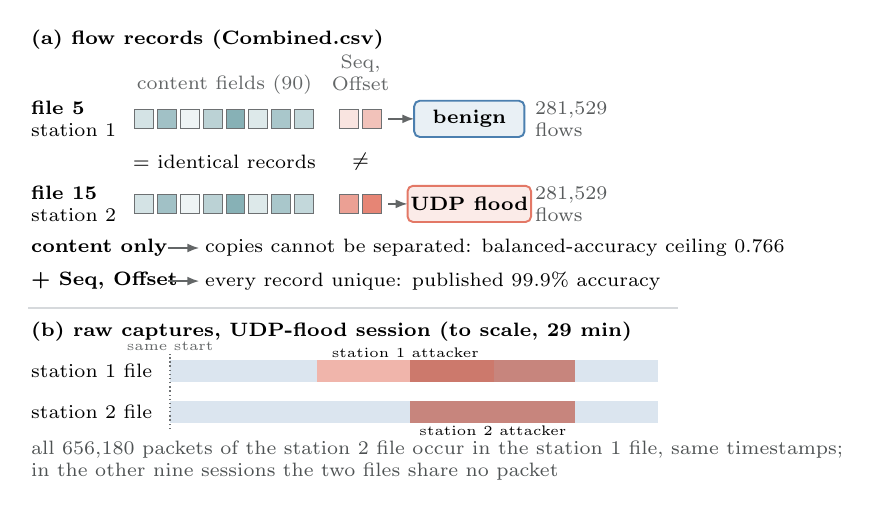
\begin{tikzpicture}[figbase, font=\scriptsize, x=1cm, y=1cm,
  tileC/.style={draw=fInk!70, line width=0.35pt, minimum size=2.4mm, inner sep=0pt},
  chipB/.style={draw=fBlue, fill=fBlue!12, rounded corners=2pt, line width=0.7pt,
                minimum width=14mm, minimum height=4.6mm, font=\scriptsize\bfseries},
  chipA/.style={draw=fCor, fill=fCor!15, rounded corners=2pt, line width=0.7pt,
                minimum width=14mm, minimum height=4.6mm, font=\scriptsize\bfseries},
  arr/.style  ={-{Latex[length=1.5mm]}, draw=fInk!75, line width=0.6pt},
]
\def\shades{25,55,10,40,70,20,50,35}
\newcommand{\fcRecord}[3]{% y, first position shade, second position shade
  \foreach \s [count=\i] in \shades
    {\node[tileC, fill=fTeal!\s] at ({1.42+0.29*(\i-1)},#1) {};}
  \node[tileC, fill=fCor!#2] at (4.02,#1) {};
  \node[tileC, fill=fCor!#3] at (4.31,#1) {};}

% ---- panel a: records ------------------------------------------------------
\node[anchor=west, font=\scriptsize\bfseries] at (-0.05,5.42) {(a) flow records (Combined.csv)};
\node[text=fInk!75] at (2.44,4.86) {content fields (90)};
\node[text=fInk!75, align=center] at (4.17,5.00) {Seq,\\Offset};

\node[anchor=west, align=left] at (-0.05,4.42) {\textbf{file \LcBenignFile}\\station 1};
\fcRecord{4.42}{20}{45}
\node[chipB] (lb) at (5.55,4.42) {benign};
\draw[arr] (4.52,4.42) -- (lb.west);
\node[anchor=west, align=left, text=fInk!80] at (6.35,4.42) {\RCopies{}\\flows};

\node[anchor=west, align=left] at (-0.05,3.34) {\textbf{file \LcAttackFile}\\station 2};
\fcRecord{3.34}{70}{90}
\node[chipA] (la) at (5.55,3.34) {UDP flood};
\draw[arr] (4.52,3.34) -- (la.west);
\node[anchor=west, align=left, text=fInk!80] at (6.35,3.34) {\RCopies{}\\flows};

\node[fill=white, inner sep=1pt] at (2.44,3.88) {$=$ identical records};
\node[fill=white, inner sep=1pt] at (4.17,3.88) {$\neq$};

\node[anchor=west, font=\scriptsize\bfseries] at (-0.05,2.78) {content only};
\draw[arr] (1.72,2.78) -- (2.12,2.78);
\node[anchor=west, align=left] at (2.16,2.78)
     {copies cannot be separated: balanced-accuracy ceiling \LcCeilNative{}};
\node[anchor=west, font=\scriptsize\bfseries] at (-0.05,2.36) {+ Seq, Offset};
\draw[arr] (1.72,2.36) -- (2.12,2.36);
\node[anchor=west, align=left] at (2.16,2.36)
     {every record unique: published 99.9\% accuracy};
\draw[draw=fgRule, line width=0.5pt] (-0.05,2.02) -- (8.20,2.02);

% ---- panel b: raw captures, TO SCALE --------------------------------------------
% x = 1.75 + 6.2 * (t - capture start) / capture length, from
% results/EXP-072/summary.json: the station-1 attacker 10.155.15.4 floods from
% x = 3.617 to 5.859, the station-2 attacker 10.155.15.7 from 4.803 to 6.898.
\node[anchor=west, font=\scriptsize\bfseries] at (-0.05,1.72) {(b) raw captures, UDP-flood session (to scale, 29 min)};
% station 1 file: both attackers' packets
\node[anchor=west] at (-0.05,1.22) {station 1 file};
\fill[fBlue!20] (1.75,1.08) rectangle (7.95,1.36);
\fill[fCor!55] (3.617,1.08) rectangle (5.859,1.36);
\fill[fCor!85!black, opacity=0.75] (4.803,1.08) rectangle (6.898,1.36);
% station 2 file: station 2's packets only
\node[anchor=west] at (-0.05,0.70) {station 2 file};
\fill[fBlue!20] (1.75,0.56) rectangle (7.95,0.84);
\fill[fCor!85!black, opacity=0.75] (4.803,0.56) rectangle (6.898,0.84);
\draw[densely dotted, fInk!70, line width=0.5pt] (1.75,0.48) -- (1.75,1.44);
\node[font=\tiny, text=fInk!75, anchor=south] at (1.75,1.44) {same start};
\node[font=\tiny, anchor=south] at (4.738,1.36) {station 1 attacker};
\node[font=\tiny, anchor=north] at (5.850,0.56) {station 2 attacker};
\node[anchor=west, align=left, text=fInk!85] at (-0.05,0.08)
     {all \RPcapBSTwoPkts{} packets of the station 2 file occur in the station 1 file,
      same timestamps;\\in the other nine sessions the two files share no packet};
\end{tikzpicture}
}
\caption{The label conflict in 5G-NIDD. Top: identical flow records occur in two capture files, labeled benign in station~1's file and UDP flood in station~2's (schematic tiles). They differ only in the row index and the record-position fields \texttt{Seq} and \texttt{Offset}, which make almost every record unique, account for the published 99.9\%, and are never seen by a deployed detector. Bottom: in the raw captures of this session, station~1's file contains every packet of station~2's file with the same timestamp; in the other nine sessions the two files share no packet.}
\label{fig:conflict}
\end{figure}

\emph{What the copies do to a classifier.} Identical records under opposite labels cap any classifier that reads only record content: even on the flows it was built from, the best function of the \LcNFeat{} content fields reaches a balanced accuracy of \LcCeilNative{}, and of the 18 shared columns \LcCeilShared{}. With \texttt{Seq} and \texttt{Offset}, almost every record becomes unique and the ceiling rises to \LcCeilPos{}.

\emph{A published result under the same protocols.} The dataset authors report binary accuracies of 99.85\% to 99.95\% on a random 70/30 split~\cite{samarakoon2022niddarxiv,siriwardhana2025descriptor}. We rebuilt their pipeline (the published one-hot encoding, the ten features with the highest ANOVA $F$-scores, $z$-score normalization, and their five classifiers with scikit-learn defaults, as tuned values are not reported) and obtain \PubRzAccMin\% to \PubRzAccMax\% for DT, RF, KNN, and the MLP (Table~\ref{tab:ladder}). Their two top features are \texttt{Seq} and \texttt{Offset}, which no deployed detector observes and which are exactly what separates the conflicting records. Replacing only these two fields with the next two in the ranking brings the accuracy of DT, RF, and the MLP down to \PubOneNoposAccMin\% to \PubOneNoposAccMax\% (balanced accuracy \PubOneNoposBAmin{} to \PubOneNoposBAmax), yet RF still reaches \PubOneRFclean{} on the flows without the copies. With capture files held out, the published features give balanced accuracies of \PubTwoPubBAmin{} to \PubTwoPubBAmax{} and, without the two fields, \PubTwoNoposBAmin{} to \PubTwoNoposBAmax{}; accuracy falls to \PubTwoNoposFoldAccMin\% on the split that trains on one UDP-flood file and tests on the other. Across base stations the published features give \PubThreePubBAmin{} to \PubThreePubBAmax{}. A 99.9\% accuracy on this corpus says little about a new capture file or base station, and nothing about a deployment, where record positions do not exist.

\begin{table*}[t]
\caption{The 5G-NIDD authors' pipeline~\cite{samarakoon2022niddarxiv,siriwardhana2025descriptor} reproduced and moved one protocol at a time (R0: their protocol). Balanced accuracy on all flows, and for RF also balanced accuracy and false positive rate without the benign-labeled copies. Mean over two repetitions per rung. KNN runs at R0 only, as its prediction dominated the runtime on later rungs.}
\label{tab:ladder}
\centering
\footnotesize
% GENERATED by analysis/make_tables.py on 2026-09-26
% source: EXP-052 published_ladder (EXP-055)
% commit: 30327c2
% DO NOT EDIT. Edit the generator, then re-run `make tables`.
\begin{tabular}{lllccccccc}
\toprule
& & & \multicolumn{5}{c}{Balanced accuracy, all flows} & \multicolumn{2}{c}{RF, w/o copies} \\
Rung & Split & Features & DT & RF & KNN & NB & MLP & BA & FPR \\
\midrule
R0 & Random 70/30 & Published 10 & 0.9995 & 0.9996 & 0.9988 & 0.9310 & 0.9986 & 0.9997 & 0.0003 \\
R1 & Random 70/30 & No \texttt{Seq}/\texttt{Offset} & 0.7059 & 0.7059 & -- & 0.6814 & 0.7042 & 0.9999 & 0.0003 \\
R2 & Capture file & Published 10 & 0.8594 & 0.9226 & -- & 0.7501 & 0.8669 & 0.9578 & 0.0018 \\
R2 & Capture file & No \texttt{Seq}/\texttt{Offset} & 0.7988 & 0.7996 & -- & 0.7593 & 0.8004 & 0.8958 & 0.0013 \\
R3 & Base station & Published 10 & 0.7619 & 0.8949 & -- & 0.6598 & 0.8577 & 0.9354 & 0.0009 \\
R3 & Base station & No \texttt{Seq}/\texttt{Offset} & 0.6557 & 0.6555 & -- & 0.6271 & 0.6919 & 0.8284 & 0.0007 \\
\bottomrule
\end{tabular}

\end{table*}

\subsection{Transfer Across Corpora}
\label{sec:res:transfer}

Table~\ref{tab:transfer} and Fig.~\ref{fig:transfer} give the transfer from \DA{} to \DB{}, with the byte correction, over 20 splits. On all flows, with the published labels, balanced accuracy falls from \RSrcBAmin{} to \RSrcBAmax{} on held-out source data to \RTrAllBAmin{} to \RTrAllBAmax{} on \DB{}, a loss that is significant after Holm correction for \RTrAllSigNbN{} of the six architectures. Much of this loss is the label conflict: a detector that has learned to recognize a UDP flood on \DA{} also flags the benign-labeled copies in file~\LcBenignFile{}.

On the clean flows, target balanced accuracy is \RTrCleanBAmin{} to \RTrCleanBAmax. The four tree-based architectures score as well on \DB{} as on held-out \DA{}: their target balanced accuracy is \RTrTreeCleanBAmin{} to \RTrTreeCleanBAmax{}, and their loss against held-out source data is \RTrTreeCleanDmin{} to \RTrTreeCleanDmax{}, none of it significant. LR and the MLP transfer worst (\RTrLRCleanBA{} and \RTrMLPCleanBA), and only the loss of LR is significant after Holm correction. Relabeling the copies as attack, which keeps every flow of \DB{}, gives the same picture (\RTrRelabBAmin{} to \RTrRelabBAmax). The label conflict reverses the ranking of the architectures: LR, which flags almost none of the copies, looks best on all flows and is worst on consistent labels. Without the byte correction, our first analysis of the same flows had found \RPrevCleanOthMin{} to \RPrevCleanOthMax{} for the five nonlinear architectures; with it, the tree-based models reach \RTrTreeCleanBAmin{} to \RTrTreeCleanBAmax{}, while the MLP falls to \RTrMLPCleanBA.

The source score is not the right yardstick, however, because \DB{} is easier than held-out \DA{}. Trained on \DB{} itself, the same architectures reach \RRefRandCleanmin{} to \RRefRandCleanmax{} on a random split and \RRefLofoCleanmin{} to \RRefLofoCleanmax{} when every capture file is held out once. On the same flows, transfer falls \RGapCleanMin{} to \RGapCleanMax{} short of this leave-one-capture-file-out reference (Table~\ref{tab:transfer}). The shortfall is significant after Holm correction for \RGapCleanSigN{} of the six architectures; for the others the intervals are wide, because target balanced accuracy varies much between splits, which train on different source addresses. Trained on one base station and tested on the other, the reference still reaches \RRefSoneCleanmin{} to \RRefSoneCleanmax{} from station~1 to station~2 and \RRefStwoCleanmin{} to \RRefStwoCleanmax{} in the other direction, so a model trained on 5G-NIDD traffic carries over to the other base station far better than one trained on \DA{} carries over to 5G-NIDD.

\begin{table*}[t]
\caption{Transfer from \DA{} to \DB{} (5G-NIDD) in the shared space with the byte correction, mean over 20 splits. All flows: published labels. Clean: the benign-labeled flood copies removed. Relabeled: the copies labeled as attack. $\Delta_{\mathrm{BA}}$: held-out source minus target balanced accuracy. Reference: models trained on \DB{} with each capture file held out once (LOFO), evaluated on the same clean flows; Ref.$-$transfer is the shortfall of transfer. Brackets: Nadeau--Bengio corrected 95\% intervals over the 20 splits (group-count ratio), unadjusted; $^{\ast}$: significant after Holm correction across the six architectures. Italic rows: input-blind baselines.}
\label{tab:transfer}
\centering
\footnotesize
\setlength{\tabcolsep}{3.2pt}
\begin{tabular}{lcccccccc}
\toprule
 & Source & All flows & \multicolumn{2}{c}{Clean} & \multicolumn{2}{c}{Relabeled} & \multicolumn{2}{c}{Reference (LOFO), clean} \\
\cmidrule(lr){4-5}\cmidrule(lr){6-7}\cmidrule(lr){8-9}
Model & BA & BA & BA & $\Delta_{\mathrm{BA}}$ [95\% CI] & BA & $\Delta_{\mathrm{BA}}$ [95\% CI] & BA & Ref.$-$transfer [95\% CI] \\
\midrule
LR & 0.837 & 0.631 & 0.613 & +0.223$^{\ast}$ [0.11, 0.33] & 0.574 & +0.263$^{\ast}$ [0.15, 0.37] & 0.959 & +0.345$^{\ast}$ [0.33, 0.36] \\
DT & 0.822 & 0.569 & 0.781 & +0.042 [$-$0.17, 0.25] & 0.802 & +0.020 [$-$0.20, 0.24] & 0.974 & +0.194 [0.00, 0.39] \\
RF & 0.808 & 0.592 & 0.818 & $-$0.010 [$-$0.27, 0.25] & 0.836 & $-$0.028 [$-$0.29, 0.23] & 0.975 & +0.157 [$-$0.02, 0.33] \\
XGB & 0.865 & 0.588 & 0.858 & +0.007 [$-$0.23, 0.24] & 0.886 & $-$0.020 [$-$0.26, 0.22] & 0.975 & +0.117 [0.00, 0.23] \\
HGB & 0.867 & 0.584 & 0.860 & +0.007 [$-$0.19, 0.20] & 0.890 & $-$0.023 [$-$0.22, 0.17] & 0.976 & +0.115$^{\ast}$ [0.07, 0.16] \\
MLP & 0.903 & 0.521 & 0.688 & +0.215 [$-$0.05, 0.48] & 0.715 & +0.188 [$-$0.08, 0.46] & 0.973 & +0.285$^{\ast}$ [0.07, 0.50] \\
\textit{Strat.} & 0.502 & 0.500 & -- & -- & -- & -- & -- & -- \\
\textit{Maj.} & 0.500 & 0.500 & -- & -- & -- & -- & -- & -- \\
\bottomrule
\end{tabular}

\end{table*}

\begin{figure}[t]
\centering
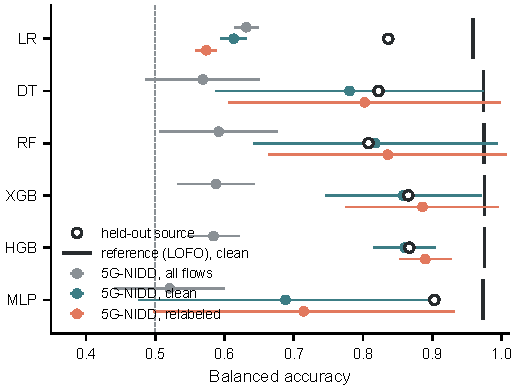
\includegraphics[width=\columnwidth]{figs/fig_transfer}
\caption{Balanced accuracy of detectors trained on \DA{}, on held-out \DA{} (open circles) and on \DB{} (filled, with corrected 95\% interval over 20 splits) for all flows, clean flows, and with the copies relabeled. Vertical bar: the reference trained on \DB{} with each capture file held out, on the clean flows. On consistent labels the tree-based models score as well on \DB{} as on held-out \DA{}, but well below what \DB{} itself allows.}
\label{fig:transfer}
\end{figure}

\emph{A third corpus.} From \DA{} to \DC{} (Table~\ref{tab:third}, 20 splits), balanced accuracy is \RTrCAllBAmin{} to \RTrCAllBAmax{} and ROC-AUC \RTrCAllAUCmin{} to \RTrCAllAUCmax{}; the loss against held-out source data is not significant for any architecture. Inside \DC{}, the same architectures reach \ThRefShRandBAmin{} to \ThRefShRandBAmax{} on a random split and \ThRefShLofoBAmin{} to \ThRefShLofoBAmax{} when the capture file of one attack type is held out. Every architecture detects the SYN flood, which training contained (recall \RCSynMax{} for all six), whereas recall on the ICMP flood is \RCIcmpMin{} to \RCIcmpMax{} and on the PFCP attack, an attack type absent from \DA{}, \RCPfcpMin{} to \RCPfcpMax. Most errors come from the benign traffic of the new site: the false positive rate is \RCFPRmin{} to \RCFPRmax{}, and up to \RCBkgMax{} of the core network's own signaling is flagged. In the reverse direction, models trained on \DB{} reach \RRevABAmin{} to \RRevABAmax{} on \DA{} and \RRevCBAmin{} to \RRevCBAmax{} on \DC{}.

\begin{table*}[t]
\caption{Transfer to the third corpus \DC{} (5G core testbed, NFStream flows with Ethernet and GTP-U bytes removed~\cite{nugraha2025fivegdatasets}): balanced accuracy on held-out source data and on \DC{}, target ROC-AUC, recall per attack type, and the share of the core's own signaling flagged (Bkg.), at $\tau = 0.5$. Mean over 20 splits from \DA{} and 20 from \DB{} (split by capture file).}
\label{tab:third}
\centering
\footnotesize
\begin{tabular}{lccccccccc}
\toprule
 & \multicolumn{7}{c}{Trained on \DA{}} & \multicolumn{2}{c}{Trained on \DB{}} \\
\cmidrule(lr){2-8}\cmidrule(lr){9-10}
Model & Src.\ BA & Tgt.\ BA & AUC & SYN & ICMP & PFCP & Bkg. & Tgt.\ BA & AUC \\
\midrule
LR & 0.837 & 0.742 & 0.800 & 1.00 & 0.10 & 0.00 & 0.27 & 0.552 & 0.708 \\
DT & 0.822 & 0.658 & 0.696 & 1.00 & 1.00 & 0.79 & 0.67 & 0.603 & 0.612 \\
RF & 0.808 & 0.596 & 0.926 & 1.00 & 1.00 & 0.99 & 0.81 & 0.699 & 0.855 \\
XGB & 0.865 & 0.640 & 0.892 & 1.00 & 1.00 & 0.72 & 0.70 & 0.584 & 0.765 \\
HGB & 0.867 & 0.698 & 0.932 & 1.00 & 1.00 & 0.80 & 0.61 & 0.726 & 0.773 \\
MLP & 0.903 & 0.677 & 0.830 & 1.00 & 0.20 & 0.63 & 0.47 & 0.811 & 0.739 \\
\bottomrule
\end{tabular}

\end{table*}

\subsection{What the Gap Consists Of, and Adaptation}
\label{sec:res:gap}

\emph{Byte accounting and separability.} Removing the Ethernet header changed what the shift diagnostics say. A domain classifier (histogram gradient boosting, five-fold cross-validation) tells \DA{} from \DB{} flows with a balanced accuracy of \RDomArgShared{} on the 18 shared columns, but \RDomArgRobust{} on the nine exporter-robust columns, against \RDomOldRobust{} before the correction: the uncorrected header had made the mean packet sizes of the two corpora almost perfectly separable. The robust columns still shift as much as the others ($\bar{W}_1$ of \RWoneArgRobust{} against \RWoneArgNonrobust{} after a quantile map fitted on source data; Fig.~\ref{fig:shift}). The correction did not shrink this shift: most \DB{} flows are UDP and most \DA{} flows TCP, and a 28-byte UDP packet now lies where \DA{} has few packets, whereas the uncorrected 42 bytes had placed it among the 40- to 44-byte TCP packets of \DA{}. The remaining shift is a difference in traffic composition, which no byte accounting removes.

\begin{figure}[t]
\centering
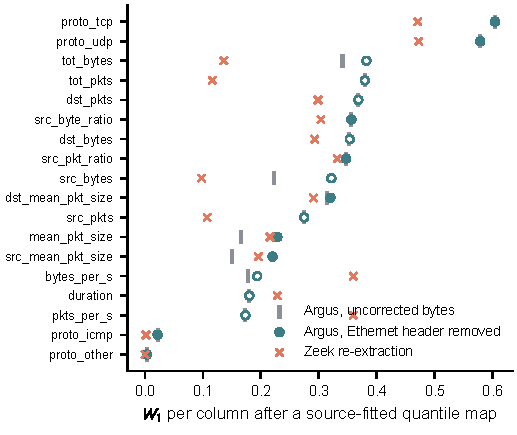
\includegraphics[width=\columnwidth]{figs/fig_shift}
\caption{Covariate shift between \DA{} and \DB{} per shared column: first-order Wasserstein distance after a quantile map fitted on \DA{} training data. Bars: Argus flows before the byte correction; circles: after it (filled: exporter-robust subset); crosses: our Zeek re-extraction of the 5G-NIDD captures. The correction moves the packet-size columns but does not remove the shift.}
\label{fig:shift}
\end{figure}

\emph{A common exporter.} The raw captures of \DB{} are public, so we re-extracted them with Zeek~(version \ZkVersion{}), the exporter family of \DA{}, and labeled each flow by the attack host pairs of its capture file, a rule that reproduces \ZkRuleAgreePct\% of the published labels on the Argus flows. Scored by the same trained models, the clean Zeek flows reach \RZkTreeCleanBAmin{} to \RZkTreeCleanBAmax{} for the tree-based architectures, \RZkTreeCleanDiffMin{} to \RZkTreeCleanDiffMax{} relative to the corrected Argus flows, and the domain classifier separates \DA{} from the Zeek flows as well as from the Argus flows (\RDomZkShared{} on all columns, \RDomZkRobust{} on the robust ones). Our Zeek configuration may differ from the undocumented one behind \DA{} in timeouts or single-packet handling, so this comparison cannot separate traffic composition from exporter configuration.

\emph{Feature subset and adaptation without target labels.} Table~\ref{tab:arms} tests whether other inputs or adaptation methods close the gap. Restricting the models to the nine exporter-robust columns raises held-out source balanced accuracy for five architectures but lowers it for LR (\RArmRobLRSrc{} against \RArmPlainLRSrc). On the clean target flows, XGB and HGB keep their level (\RArmRobXGBClean{} and \RArmRobHGBClean), whereas DT and RF fall to \RArmRobDTClean{} and \RArmRobRFClean: the columns that an exporter moves least are not enough. None of the three adaptation methods that read unlabeled target flows beats the plain tree-based models. Importance weighting changes little (\RArmIwTreeCleanMin{} to \RArmIwTreeCleanMax{} for the tree-based models), because its domain classifier separates the corpora so well that the weights concentrate on \RIwESSmin\% to \RIwESSmax\% of the source flows in effective sample size. CORAL raises the MLP from \RArmPlainMLPClean{} to \RArmCoralMLPClean{} but pushes the target false positive rate of the tree-based models to \RArmCoralTreeFPRmin{} to \RArmCoralTreeFPRmax, as in our first analysis. Domain-adversarial training reaches \RArmDannDANNClean.

\begin{table}[t]
\caption{Transfer from \DA{} to \DB{} under other feature sets and with adaptation, mean over 20 splits, at $\tau = 0.5$. Importance weighting, CORAL, and DANN read unlabeled target flows. Clean: the benign-labeled copies removed; relab.: the copies labeled as attack.}
\label{tab:arms}
\centering
\scriptsize
\setlength{\tabcolsep}{2.6pt}
\input{tables/arms}
\end{table}

\emph{A few labeled target captures.} Labeled data from the target helps far more (Fig.~\ref{fig:labeleff}). Added to the \DA{} training data, a single labeled capture file of \DB{} raises the balanced accuracy of the five nonlinear architectures on the capture files not drawn to \RLeSrcOneNlMin{} to \RLeSrcOneNlMax{} (the MLP from \RLeZeroMLP{} to \RLeSrcOneMLP), close to the leave-one-capture-file-out reference, and eight files to \RLeSrcEightNlMin{} to \RLeSrcEightNlMax. The same capture files alone give only \RLeTgtOneNlMin{} to \RLeTgtOneNlMax{} for one file, so the source data still carries most of what the detectors know. The alert bound takes more data. With the threshold fixed on source data, the six architectures met all three alert conditions in \RLeSrcOneMeet{} of \RLeSrcOneCells{} draws with one labeled file and in \RLeSrcEightMeet{} of \RLeSrcEightCells{} with eight; with eight files, XGB and the MLP met them in every draw, at \RLeSrcEightXGBAlerts{} and \RLeSrcEightMLPAlerts{} false alerts per hour on average and a recall of about \RLeSrcEightXGBRecall.

\begin{figure*}[t]
\centering
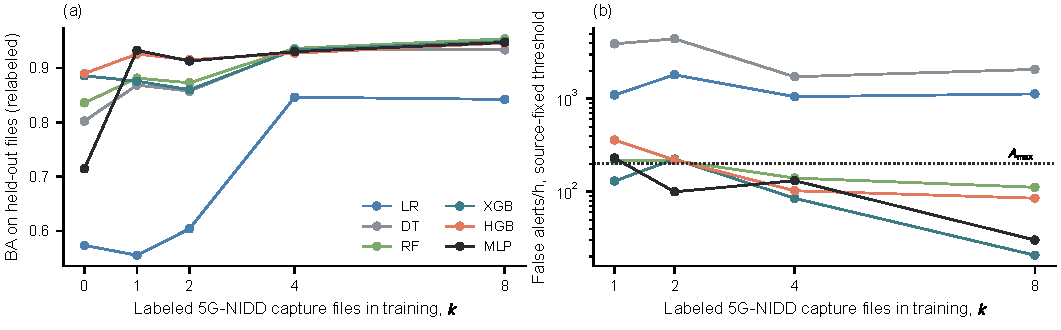
\includegraphics[width=0.92\textwidth]{figs/fig_label_efficient}
\caption{Label-efficient arm: $k$ labeled capture files of \DB{} added to the \DA{} training data (four random draws per $k$; $k = 0$ is the plain transfer of the 20 splits), evaluated on the capture files not drawn, with the copies relabeled as attack. (a) Balanced accuracy; (b) false alerts per hour at the threshold fixed on source data, mean over draws, with the bound $A_{\max}$.}
\label{fig:labeleff}
\end{figure*}

\emph{Size of the source sample.} Repeating the transfer with \RSzNlist{} source flows (\RSzSplits{} splits, five architectures) changed clean target balanced accuracy by at most \RSzMaxChangeClean{} against \NSub{} flows, in no consistent direction, which is within the variation between splits.


\subsection{Alert Burden and the Deployability Test}
\label{sec:res:alerts}

\emph{Alert volumes.} At the default threshold of 0.5, the transferred detectors raise many false alerts. On the clean flows of \DB{}, their false positive rate is \ROpBCleanFPRmin{} to \ROpBCleanFPRmax, that is, \ROpBCleanAlertsMin{} to \ROpBCleanAlertsMax{} false alerts per hour at our declared rate, for an operational precision of \ROpBCleanPPVmin{} to \ROpBCleanPPVmax{} at $\pi = 0.002$. On all flows, where the copies count as benign, the false positive rate reaches \ROpBAllFPRmax.

\emph{The test.} Table~\ref{tab:test} applies the two-term test of Section~\ref{sec:crit:test}. No detector passes in any label view. On all flows, \RTestAllFailN{} of the six detectors fail and \RTestAllInconclusiveN{} is inconclusive. On the clean flows, the generalization term fails for LR and is inconclusive for the other \RTestCleanGenInconclusiveN{} architectures: their intervals include losses larger than $\delta$, so neither a pass nor a failure is established. The alert term fails for \RTestCleanAlertFailN{} architectures and is inconclusive for \RTestCleanAlertInconclusiveN{}. Its intervals are wide because the threshold fixed on the source data of each split lands differently on the target: across the 20 splits, one architecture can range from no alerts, and no detections, to tens of thousands of false alerts per hour. Counted split by split, HGB meets all three alert conditions in \RJointHGBClean{} of the 20 splits, the MLP in \RJointMLPClean{}, XGB in \RJointXGBClean{}, and the other architectures in none. Averaged over the splits, HGB raises \RTestHGBCleanAlerts{} false alerts per hour at a recall of \RTestHGBCleanRecall{} and an operational precision of \RTestHGBCleanPPV{}, more alerts than our bound allows. Relabeling the copies gives the same verdicts except for RF, whose alert term becomes inconclusive.

\begin{table*}[t]
\caption{Two-term deployability test (Section~\ref{sec:crit:test}) for transfer from \DA{} to \DB{}, 20 splits. Generalization: $\Delta_{\mathrm{BA}}$ with its Nadeau--Bengio corrected 95\% interval; pass if the upper bound is at most $\delta = 0.10$, fail if the lower bound exceeds it. Alert burden at the threshold fixed on each split's held-out source data (recall at least 0.5 there): mean recall, false alerts per hour at $\lambda_b = 240{,}000$ benign flows per hour, and operational precision at $\pi = 0.002$, with corrected intervals; pass if all three intervals lie on the passing side of $r_{\min} = 0.5$, $A_{\max} = 200$, and $\rho = 0.1$, fail if any lies on the failing side. Splits: splits in which all three alert conditions hold. $\checkmark$: pass, $\times$: fail, ?: inconclusive; $\mathcal{P}$: verdict. The bounds are our own, not operator requirements.}
\label{tab:test}
\centering
\scriptsize
\setlength{\tabcolsep}{3pt}
\begin{tabular}{llcccccccc}
\toprule
 & & \multicolumn{2}{c}{Generalization} & \multicolumn{5}{c}{Alert burden, threshold fixed on source data} & \\
\cmidrule(lr){3-4}\cmidrule(lr){5-9}
View & Model & $\Delta_{\mathrm{BA}}$ [95\% CI] & & Recall [95\% CI] & Alerts/h [95\% CI] & PPV [95\% CI] & Splits & & $\mathcal{P}$ \\
\midrule
All flows & LR & +0.21 [0.10, 0.31] & ? & 0.04 [0.00, 0.09] & 570 [0, 1{,}832] & 0.032 [0.000, 1.000] & 0/20 & $\times$ & $\times$ \\
 & DT & +0.25 [0.06, 0.45] & ? & 0.70 [0.41, 0.98] & 146{,}512 [88{,}607, 204{,}416] & 0.002 [0.001, 0.005] & 0/20 & $\times$ & $\times$ \\
 & RF & +0.22 [$-$0.02, 0.46] & ? & 0.14 [0.00, 0.47] & 31{,}967 [0, 107{,}201] & 0.002 [0.000, 1.000] & 0/20 & $\times$ & $\times$ \\
 & XGB & +0.28 [0.07, 0.48] & ? & 0.19 [0.00, 0.58] & 45{,}441 [0, 137{,}454] & 0.002 [0.000, 1.000] & 0/20 & ? & ? \\
 & HGB & +0.28 [0.10, 0.47] & ? & 0.51 [0.16, 0.86] & 113{,}355 [38{,}968, 187{,}742] & 0.002 [0.000, 0.011] & 0/20 & $\times$ & $\times$ \\
 & MLP & +0.38 [0.22, 0.55] & $\times$ & 0.39 [0.00, 0.84] & 85{,}583 [0, 189{,}405] & 0.002 [0.000, 1.000] & 0/20 & ? & $\times$ \\
\midrule
Clean & LR & +0.22 [0.11, 0.33] & $\times$ & 0.04 [0.00, 0.09] & 1{,}387 [0, 4{,}460] & 0.014 [0.000, 1.000] & 0/20 & $\times$ & $\times$ \\
 & DT & +0.04 [$-$0.17, 0.25] & ? & 0.70 [0.41, 0.98] & 46{,}906 [0, 127{,}390] & 0.007 [0.002, 1.000] & 0/20 & ? & ? \\
 & RF & $-$0.01 [$-$0.27, 0.25] & ? & 0.14 [0.00, 0.47] & 101 [0, 511] & 0.406 [0.000, 1.000] & 0/20 & $\times$ & $\times$ \\
 & XGB & +0.01 [$-$0.23, 0.24] & ? & 0.19 [0.00, 0.58] & 41 [0, 259] & 0.691 [0.000, 1.000] & 2/20 & ? & ? \\
 & HGB & +0.01 [$-$0.19, 0.20] & ? & 0.51 [0.16, 0.86] & 352 [0, 2{,}845] & 0.412 [0.027, 1.000] & 12/20 & ? & ? \\
 & MLP & +0.21 [$-$0.05, 0.48] & ? & 0.39 [0.00, 0.84] & 1{,}762 [0, 7{,}043] & 0.096 [0.000, 1.000] & 4/20 & ? & ? \\
\midrule
Relabeled & LR & +0.26 [0.15, 0.37] & $\times$ & 0.03 [0.00, 0.06] & 1{,}387 [0, 4{,}460] & 0.010 [0.000, 1.000] & 0/20 & $\times$ & $\times$ \\
 & DT & +0.02 [$-$0.20, 0.24] & ? & 0.75 [0.45, 1.00] & 46{,}906 [0, 127{,}390] & 0.008 [0.002, 1.000] & 0/20 & ? & ? \\
 & RF & $-$0.03 [$-$0.29, 0.23] & ? & 0.17 [0.00, 0.55] & 101 [0, 511] & 0.442 [0.000, 1.000] & 0/20 & ? & ? \\
 & XGB & $-$0.02 [$-$0.26, 0.22] & ? & 0.23 [0.00, 0.69] & 41 [0, 259] & 0.728 [0.000, 1.000] & 2/20 & ? & ? \\
 & HGB & $-$0.02 [$-$0.22, 0.17] & ? & 0.59 [0.20, 0.99] & 352 [0, 2{,}845] & 0.448 [0.032, 1.000] & 12/20 & ? & ? \\
 & MLP & +0.19 [$-$0.08, 0.46] & ? & 0.45 [0.00, 0.98] & 1{,}762 [0, 7{,}043] & 0.109 [0.000, 1.000] & 4/20 & ? & ? \\
\bottomrule
\end{tabular}

\end{table*}

\emph{An optimistic bound.} A threshold searched on the target shows what the ranking itself allows. With the best such threshold, HGB reaches an operational precision of \ROracleHGBCleanPPV{} at \ROracleHGBCleanAlerts{} false alerts per hour on the clean flows, and XGB \ROracleXGBCleanPPV{} at \ROracleXGBCleanAlerts{}, both within our bounds; \RTestCleanOracleN{} architectures meet the bounds in this way, and none does on all flows, where the best operational precision at a recall of at least 0.5 is \RTestAllOraclePPVmax. On consistent labels the best transferred detectors therefore rank the attacks of \DB{} well enough for our bounds, but the threshold that would realize this cannot be chosen from source data. In our experiments the threshold, not only the model, had to be set with labeled data from the target.

\begin{figure*}[t]
\centering
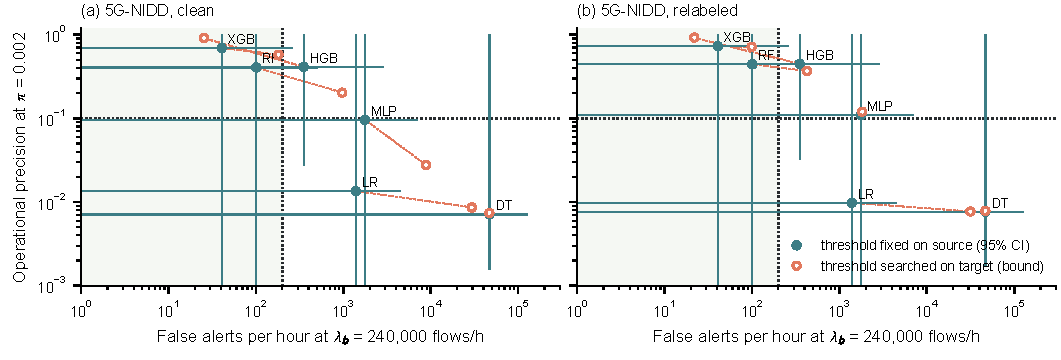
\includegraphics[width=0.92\textwidth]{figs/fig_test}
\caption{Where the transferred detectors lie relative to the alert bounds on \DB{}: false alerts per hour against operational precision, mean over 20 splits, at the threshold fixed on source data (filled, with corrected 95\% intervals) and at the best threshold searched on the target (open, an optimistic bound), for (a) clean flows and (b) copies relabeled. The shaded region meets $A_{\max} = 200$ false alerts per hour; dotted lines mark $A_{\max}$ and $\rho = 0.1$. Both bounds are our own choices; another operator would move the lines.}
\label{fig:test}
\end{figure*}

\emph{Sensitivity to the bounds.} The bounds are our own, and Fig.~\ref{fig:test} shows how far each detector lies from them. On all flows no threshold comes close: even the threshold searched on the target leaves every architecture with at least \RTestAllOracleAlertsMin{} false alerts per hour at a recall of 0.5. On consistent labels the verdict depends on the threshold rule more than on the bounds. At the threshold fixed on source data, the recall interval of every architecture extends below $r_{\min} = 0.5$, so no change of $A_{\max}$ or $\rho$ alone would make the alert term pass, and the generalization term would remain inconclusive unless $\delta$ were raised to \RTestCleanGenHiMin, the smallest upper bound of $\Delta_{\mathrm{BA}}$ on these flows.

\subsection{Radio-Layer Protocol Sensitivity}
\label{sec:res:radio}

Table~\ref{tab:radio} compares a random and a group-disjoint split on the radio layer of \DA{}, with the 30 capture sessions or the 42 experiment runs as groups; a third protocol, which keeps every attack category on both sides, gives the same picture (repository). Grouped by sessions, a random split raises macro-$F_1$ over a group-disjoint split by \RRadSessMin{} to \RRadSessMax{} across the six architectures, \RRadSessAvg{} on average. This gain is not statistically significant: the corrected interval of the average gain is \RRadSessLo{} to \RRadSessHi{} ($p = \RRadSessP$), and no architecture's gain is significant after Holm correction. Grouped by runs, the average gain is \RRadRunAvg{}, with a corrected interval of \RRadRunLo{} to \RRadRunHi{} ($p = \RRadRunP$), and again no architecture's gain is significant after Holm correction. The input-blind baselines gain nothing under either grouping, so class composition does not move macro-$F_1$ between protocols. A model-free probe is consistent with recognition of capture groups: under a random split, \RRadNNSame\% of the test windows have their nearest training window in the same session, although windows share no records, and a one-nearest-neighbor lookup reaches a macro-$F_1$ of \RRadNNRand{}, against \RRadNNGd{} under a session-disjoint split. The probe shows that recognizing the group is available to a model, not that the trained models rely on it.

\begin{table}[t]
\caption{Radio-layer protocol sensitivity on \DA{}: macro-$F_1$ under a random (R) and a group-disjoint (GD) split, with sessions (30 groups) or runs (42 groups) as the group, and the gain of the random split with its Nadeau--Bengio corrected 95\% interval (group counts), over 20 splits with two model seeds each. Intervals are unadjusted; $^{\ast}$: significant after Holm correction across the six architectures.}
\label{tab:radio}
\centering
\scriptsize
\setlength{\tabcolsep}{2.2pt}
\begin{tabular}{lcccccc}
\toprule
 & \multicolumn{3}{c}{30 sessions} & \multicolumn{3}{c}{42 runs} \\
\cmidrule(lr){2-4}\cmidrule(lr){5-7}
Model & R & GD & Gain [95\% CI] & R & GD & Gain [95\% CI] \\
\midrule
LR & 0.836 & 0.744 & +0.093 [$-$0.08, 0.26] & 0.834 & 0.738 & +0.096 [$-$0.08, 0.28] \\
DT & 0.950 & 0.782 & +0.168 [$-$0.01, 0.35] & 0.945 & 0.752 & +0.193 [0.02, 0.36] \\
RF & 0.970 & 0.853 & +0.117 [$-$0.07, 0.30] & 0.970 & 0.816 & +0.154 [$-$0.04, 0.35] \\
XGB & 0.977 & 0.836 & +0.141 [$-$0.03, 0.32] & 0.979 & 0.813 & +0.166 [$-$0.02, 0.35] \\
HGB & 0.982 & 0.844 & +0.138 [$-$0.03, 0.31] & 0.983 & 0.816 & +0.167 [$-$0.02, 0.35] \\
MLP & 0.954 & 0.828 & +0.126 [$-$0.04, 0.29] & 0.955 & 0.814 & +0.141 [$-$0.03, 0.31] \\
\textit{Strat.} & 0.498 & 0.507 & $-$0.009 [$-$0.02, 0.00] & 0.497 & 0.507 & $-$0.010 [$-$0.02, 0.00] \\
\textit{Maj.} & 0.431 & 0.434 & $-$0.002 [$-$0.02, 0.02] & 0.431 & 0.434 & $-$0.003 [$-$0.02, 0.01] \\
\midrule
Average &  &  & +0.131 [$-$0.03, 0.30] &  &  & +0.153 [$-$0.02, 0.33] \\
\bottomrule
\end{tabular}

\end{table}

The radio layer cannot support operating figures. It holds \RRadBenignWin{} benign windows, about \RRadBenignHours{} hours of data, recorded mostly with one UE and, for nine of the ten benign sessions, six weeks before the first attack session. When each benign session is held out alone (Fig.~\ref{fig:benign}), the false positive rate averaged over the six architectures is at most \BenLowMax{} for \BenLowN{} sessions and \BenHighMin{} to \BenHighMax{} for sessions \BenHighSessions{}, and a bootstrap over splits and sessions puts the pooled false positive rate between \RadCbFPRlo{} and \RadCbFPRhi{} (lowest and highest interval bound across architectures). A false positive rate this dependent on which benign session a detector meets cannot be turned into an alert rate for another network, so we report none for the radio layer.

\begin{figure}[t]
\centering
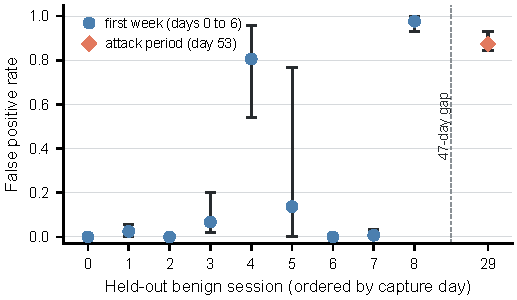
\includegraphics[width=\columnwidth]{figs/fig_benign}
\caption{False positive rate on each benign radio session of \DA{} when that session alone is held out and the models train on the other 29: mean (marker) and range (bar) over the six architectures, sessions in capture order. Within one week of capture, sessions range from no false positives to almost every window flagged, so the radio layer supports no operating figure.}
\label{fig:benign}
\end{figure}

\subsection{Decision Latency of Window-Level Detectors}
\label{sec:res:latency}

We measured latency separately, for window-level detectors only, and it is not part of the test. Our C xApp in FlexRIC v2.0.0 subscribes to E2SM-KPM reports from FlexRIC's emulated gNB over SCTP, with 16 measurement items per UE, scores every UE of a report with ONNX Runtime, answers each report with one E2SM-RC control message, and waits for the acknowledgment. The emulated node reports synthetic values, so the xApp scores held-out radio test windows in their place; the C code reproduced the Python scores on all 589 test windows to within $4\times10^{-7}$. With a report every 10\,ms (\RicNten{} reports per model), the full loop from report to acknowledged control message takes \RicLoopTenPnnMin{} to \RicLoopTenPnnMax{}\,ms at the 99th percentile over the six models (Table~\ref{tab:ric}). Delivery and control account for at least \RicTransportShareMin\% of the mean loop time, and inference takes at most \RicInfTenPnnMax{}\,ms at the 99th percentile, so once a RIC is in the path the model barely matters. At a 1\,ms period the loop ran faster (\RicLoopOnePnnMin{} to \RicLoopOnePnnMax{}\,ms), which fits a host that idles between sparse reports and pays to wake up: these are processing costs of the RIC software path on one host, under WSL2, without CPU isolation and with synthetic measurements over loopback, not the delay of a deployment.

Two limits follow. First, computation is not what limits a window-level detector: it decides once its 16\,s window is complete, so a compute tail of a few milliseconds is small next to the detection delay. Second, we have no measured latency for flow-level detectors: their records need a transport to the xApp that our loop lacks and O-RAN does not define, and the cost of a native user-plane exporter is unknown. We therefore make no latency claim for flow detectors.

\begin{table}[t]
\caption{Decision loop of a window-level detector through FlexRIC with an emulated E2 node on one host, in ms, ranges over models (one trained model per architecture, split seed 101), at a 10\,ms reporting period (six models, \RicNten{} reports each) or a 1\,ms period (LR and RF, \RicNone{} reports each). Terms of Eq.~\eqref{eq:latency}: delivery to the xApp ($t_{\mathrm{ind}}$), queueing ($t_{q}$), aggregation ($t_{\mathrm{feat}}$) and inference ($t_{\mathrm{inf}}$) for one UE, and control up to acknowledgment ($t_{\mathrm{act}}$). ``Loop'': KPM header timestamp to acknowledgment, for the first UE of a report or all its UEs.}
\label{tab:ric}
\centering
\scriptsize
\setlength{\tabcolsep}{2.4pt}
% GENERATED by analysis/make_tables.py on 2026-09-26
% source: EXP-061 ric_latency
% commit: 30327c2
% DO NOT EDIT. Edit the generator, then re-run `make tables`.
\begin{tabular}{lcccc}
\toprule
& \multicolumn{2}{c}{10\,ms, six models} & \multicolumn{2}{c}{1\,ms, LR and RF} \\
Term & $p_{50}$ & $p_{99}$ & $p_{50}$ & $p_{99}$ \\
\midrule
$t_{\mathrm{ind}}$ & 1.51--1.86 & 3.02--3.05 & 0.51--0.53 & 0.84--0.98 \\
$t_{q}$ & 0.063--0.071 & 0.18--0.21 & 0.015--0.016 & 0.069 \\
$t_{\mathrm{feat}}$ & 0.001 & 0.002--0.003 & $<$0.001 & 0.001 \\
$t_{\mathrm{inf}}$ & 0.050--0.12 & 0.13--0.23 & 0.014--0.025 & 0.038--0.050 \\
$t_{\mathrm{act}}$ & 0.72--0.87 & 1.40--1.50 & 0.20--0.21 & 0.53--0.60 \\
\midrule
Loop, 1 UE & 2.38--2.97 & 4.36--4.59 & 0.76--0.79 & 1.38--1.59 \\
Loop, all & 2.48--3.18 & 4.45--4.95 & 0.77--0.86 & 1.42--1.69 \\
\bottomrule
\end{tabular}

\end{table}

%=======================================================================
\section{Discussion}
\label{sec:discussion}

\subsection{Implications for Detection in O-RAN}
\label{sec:disc:practice}

\emph{Data path.} E2SM-KPM delivers aggregated measurements once per reporting period, not packets. A window-level detector can therefore live inside the RIC, whereas a flow-level detector needs an exporter near the user plane (in the central unit or at the user-plane function) and a way to move its records to the xApp, such as a custom E2 service model or the non-real-time data collection path. This transport adds to $t_{\mathrm{ind}}$ in Eq.~\eqref{eq:latency}, and nobody has measured it for these detectors, ourselves included.

\emph{Detection delay.} Computation is a small part of detection time. A window-level decision waits for its 16\,s window to end, and a flow-level one for the flow record, which for a long connection means an idle or active timeout. Computational latency should be reported with the KPM reporting period and the flow timeouts.

\emph{Acting on alerts.} An E2SM-RC action such as isolating or steering a UE hits a falsely accused UE as hard as a guilty one. Without labeled target data, the averaged operating points of our flow detectors met the alert bounds only at thresholds tuned on the target (Section~\ref{sec:res:alerts}). With thresholds fixed on source data they either missed most attacks, as XGB and RF did with \RTestXGBCleanAlerts{} and \RTestRFCleanAlerts{} false alerts per hour at a recall of \RTestXGBCleanRecall{} and \RTestRFCleanRecall{}, or raised hundreds to tens of thousands of false alerts per hour at our declared rate. Alerts of this quality can inform an operator, or a policy set through the A1 interface of the non-real-time RIC, but should not drive automatic control. For such detectors the 10\,ms budget matters less than detection quality: latency binds only for a detector whose alerts are good enough to act on automatically.

\emph{Admission and calibration on site.} The two-term test could serve as an admission check at a new site, given labeled traffic from it. Our label-efficient arm (Section~\ref{sec:res:gap}) suggests that a few labeled captures from the site are worth more than adaptation without labels, and the comparison of fixed and tuned thresholds (Section~\ref{sec:res:alerts}) that the operating threshold, not only the model, has to be checked on site data.

\subsection{Relation to Reported Results}

The 5G-NIDD results we cite~\cite{samarakoon2022niddarxiv,ilias2024moe5g} are in-distribution scores, and under the same split ours are as high: \PubRzAccMin\% to \PubRzAccMax\% accuracy for the reproduced pipeline, and \ThRefShRandBAmin{} to \ThRefShRandBAmax{} balanced accuracy inside \DC{}. Setting such numbers beside transfer results compares protocols, not detectors. In our experiments a held-out score under a random split did not predict performance on another corpus: on 5G-NIDD it rested on record-position fields, the published labels hid the attack traffic of the other base station, and a byte-accounting difference between exporters entered every byte column of the shared space.

%=======================================================================
\section{Limitations}
\label{sec:limitations}

\emph{Scope of the corpora.} Only NetsLab-5GORAN-IDD is an O-RAN corpus. 5G-NIDD comes from a 5G test network and the third corpus from a 5G core in Docker, with three capture files, only flood attacks and one control-plane attack, too few for cluster resampling. Three corpora show that the transfer gap recurs, not how it varies across sites. We found no other O-RAN corpus with paired radio telemetry, so the radio detectors have no transfer target, and no detector is evaluated on all criteria.

\emph{Detectors.} The six architectures are untuned shallow models with hyperparameters fixed in advance, and we tested three adaptation methods, one per family. Tuned or larger models, other adaptation methods, or detectors built for a specific deployment may transfer differently; our conclusions concern the detectors we tested.

\emph{Flow exporters.} Zeek, Argus, and NFStream produced the three corpora. We removed the link-layer and tunnel bytes that two of them count, but other exporter differences remain: where a flow ends, and the handling of single-packet flows. Re-extracting 5G-NIDD with Zeek did not reduce the gap (Section~\ref{sec:res:gap}), but the Zeek version and configuration behind NetsLab-5GORAN-IDD are undocumented and our Zeek flows take their labels through the host pairs of each capture, so this comparison cannot separate traffic composition from exporter configuration.

\emph{Target labels.} The packet-level evidence shows that station~1's UDP-flood file contains station~2's flood, but how the file was produced is not documented, and the relabeled view rests on our reading that these flows are attacks. We therefore report every 5G-NIDD result on the published labels, without the copies, and relabeled.

\emph{Radio layer.} The radio layer has 30 sessions, each benign or from one attack category, so session and category are confounded, and nine of the ten benign sessions were recorded six weeks before the attacks, mostly with one UE. The protocol comparison detects only large effects, and the radio false positive rate depends so much on the benign session that we report no radio operating figure.

\emph{Latency.} All latency figures come from one workstation without CPU isolation, and the RIC loop used an emulated E2 node with synthetic measurements over loopback SCTP. It measures the processing cost of the RIC software path for window-level detectors, not the delay of a deployment, and no flow detector was timed in the loop.

\emph{Operational parameters and the test.} The prevalence $\pi = 0.002$, the rate $\lambda_b$, and every bound of the test are our own declarations, not operator requirements. Only $\pi$ enters operational precision, and alert counts scale linearly with $\lambda_b$. An operator may weigh recall, precision, and alert volume differently, and the test ignores detection delay and the cost of a missed attack.

\emph{Statistics.} The transfer statistics vary the training set over 20 splits and keep the target fixed, so they miss the variability across capture files and other target corpora; a bootstrap over the capture files, reported in the repository, suggests that it is large. The source splits differ much in which addresses they hold out, so the corrected intervals are wide, which is why many terms of the test are inconclusive rather than decided.

%=======================================================================
\section{Reproducibility and Ethics}
\label{sec:repro}

Code, configuration, seeded splits, per-split results, the corrected 5G-NIDD labels, and the generators for every table, figure, and in-text number are at \textcolor{blue}{\url{https://github.com/adeliusa486/oran-ids-deployability}}, where one script regenerates every number from the results or re-runs each experiment from the SHA-256-verified raw corpora (\texttt{REPRODUCE.md}). \DA{}~\cite{abedzadeh2025netslab} and \DB{}~\cite{samarakoon2022nidd}, including the release with all fields and the raw captures, are distributed by their authors under CC-BY-4.0. \DC{} is available from its authors' repository~\cite{nugraha2025fivegdatasets}, which states no license, so we do not redistribute it. All traffic comes from testbed devices and test networks, and no personal data was processed. Showing where detectors fail carries a modest dual-use risk, which we judge smaller than the benefit to operators of knowing that reported accuracy need not carry over to their networks.

%=======================================================================
\section{Conclusion and Reporting Recommendations}
\label{sec:conclusion}

A held-out score on one corpus said little about how the flow detectors we tested behave on traffic from another network. In 5G-NIDD, \RCopiesPct\% of the benign flows are the UDP flood of the other base station, recorded packet for packet in station~1's capture, and a published 99.9\% accuracy rests on record-position fields that a deployed detector never sees. Once the labels and the byte accounting of the exporters are corrected, tree-based detectors trained on NetsLab-5GORAN-IDD score as well on 5G-NIDD as on held-out source data, but \RGapTreeCleanMin{} to \RGapTreeCleanMax{} below references trained on 5G-NIDD and tested on the same flows; on the 5G core testbed they catch the flood they were trained on and flag much benign traffic. At a declared prevalence of 0.002 and bounds of our own, no detector passed our two-term test. The best detectors rank the attacks of 5G-NIDD well enough for the bounds, but a threshold fixed on source data did not carry over, and none of three adaptation methods without target labels closed the gap, whereas one labeled target capture closed most of it. On the radio layer, the random-split gain was not significant under either grouping, and the latency we measured for window-level detectors in a FlexRIC loop with an emulated E2 node (99th percentile at most \RicLoopTenPnnMax{}\,ms) is a processing cost on one host, not a conformance result; flow detectors were not timed. We recommend that studies of 5G flow detectors report at least:
\begin{enumerate}
\item performance on an independently collected corpus in a prevalence-invariant metric, beside input-blind baselines and a reference trained on that corpus and tested on the same flows;
\item the split protocol and group key, and intervals that account for overlapping splits and clustered samples;
\item how each flow exporter counts bytes, and how the shared feature space removes the differences;
\item evidence that the labels are a function of the features used, such as the share of identical records under opposite labels, and that no record-position or identifier field is a feature;
\item the false positive rate with its unit, the alert rate and operational precision at a stated base rate, and whether the operating threshold was chosen with target labels;
\item for a detector meant for the RIC, the latency from indication to control acknowledgment, with stages, implementation, and host, measured with a real E2 node before any conformance claim.
\end{enumerate}




\begin{thebibliography}{99}
\providecommand{\url}[1]{#1}
\csname url@samestyle\endcsname
\providecommand{\newblock}{\relax}
\providecommand{\bibinfo}[2]{#2}
\providecommand{\BIBentrySTDinterwordspacing}{\spaceskip=0pt\relax}
\providecommand{\BIBentryALTinterwordstretchfactor}{4}
\providecommand{\BIBentryALTinterwordspacing}{\spaceskip=\fontdimen2\font plus
\BIBentryALTinterwordstretchfactor\fontdimen3\font minus
  \fontdimen4\font\relax}
\providecommand{\BIBforeignlanguage}[2]{{%
\expandafter\ifx\csname l@#1\endcsname\relax
\typeout{** WARNING: IEEEtran.bst: No hyphenation pattern has been}%
\typeout{** loaded for the language `#1'. Using the pattern for}%
\typeout{** the default language instead.}%
\else
\language=\csname l@#1\endcsname
\fi
#2}}
\providecommand{\BIBdecl}{\relax}
\BIBdecl

\bibitem{polese2023understanding}
M.~Polese, L.~Bonati, S.~D'Oro, S.~Basagni, and T.~Melodia, ``Understanding
  {O-RAN}: Architecture, interfaces, algorithms, security, and research
  challenges,'' \emph{IEEE Communications Surveys \& Tutorials}, vol.~25,
  no.~2, pp. 1376--1411, 2023. doi:
  \href{https://doi.org/10.1109/COMST.2023.3239220}{\nolinkurl{10.1109/COMST.2023.3239220}}

\bibitem{abdalla2022toward}
A.~S. Abdalla, P.~S. Upadhyaya, V.~K. Shah, and V.~Marojevic, ``Toward next
  generation open radio access networks: What {O-RAN} can and cannot do!''
  \emph{IEEE Network}, vol.~36, no.~6, pp. 206--213, 2022. doi:
  \href{https://doi.org/10.1109/MNET.108.2100659}{\nolinkurl{10.1109/MNET.108.2100659}}

\bibitem{niknam2022intelligent}
S.~Niknam, A.~Roy, H.~S. Dhillon, S.~Singh, R.~Banerji, J.~H. Reed, N.~Saxena,
  and S.~Yoon, ``Intelligent {O-RAN} for beyond {5G} and {6G} wireless
  networks,'' in \emph{Proc. IEEE Globecom Workshops (GC Wkshps)}, 2022, pp.
  215--220. doi:
  \href{https://doi.org/10.1109/GCWkshps56602.2022.10008676}{\nolinkurl{10.1109/GCWkshps56602.2022.10008676}}

\bibitem{bonati2021intelligence}
L.~Bonati, S.~D'Oro, M.~Polese, S.~Basagni, and T.~Melodia, ``Intelligence and
  learning in {O-RAN} for data-driven {NextG} cellular networks,'' \emph{IEEE
  Communications Magazine}, vol.~59, no.~10, pp. 21--27, 2021. doi:
  \href{https://doi.org/10.1109/MCOM.101.2001120}{\nolinkurl{10.1109/MCOM.101.2001120}}

\bibitem{antonakakis2017mirai}
\BIBentryALTinterwordspacing
M.~Antonakakis, T.~April, M.~Bailey, M.~Bernhard, E.~Bursztein, J.~Cochran,
  Z.~Durumeric, J.~A. Halderman, L.~Invernizzi, M.~Kallitsis, D.~Kumar,
  C.~Lever, Z.~Ma, J.~Mason, D.~Menscher, C.~Seaman, N.~Sullivan, K.~Thomas,
  and Y.~Zhou, ``Understanding the {Mirai} botnet,'' in \emph{Proc. 26th USENIX
  Security Symposium}, 2017, pp. 1093--1110. [Online]. Available:
  \url{https://www.usenix.org/conference/usenixsecurity17/technical-sessions/presentation/antonakakis}
\BIBentrySTDinterwordspacing

\bibitem{kolias2017ddos}
C.~Kolias, G.~Kambourakis, A.~Stavrou, and J.~Voas, ``{DDoS} in the {IoT}:
  {Mirai} and other botnets,'' \emph{Computer}, vol.~50, no.~7, pp. 80--84,
  2017. doi:
  \href{https://doi.org/10.1109/MC.2017.201}{\nolinkurl{10.1109/MC.2017.201}}

\bibitem{wen2024spector}
H.~Wen, P.~Porras, V.~Yegneswaran, A.~Gehani, and Z.~Lin, ``{5G-Spector}: An
  {O-RAN} compliant layer-3 cellular attack detection service,'' in \emph{Proc.
  Network and Distributed System Security Symposium (NDSS)}, 2024. doi:
  \href{https://doi.org/10.14722/ndss.2024.24527}{\nolinkurl{10.14722/ndss.2024.24527}}

\bibitem{scalingi2024detran}
A.~Scalingi, S.~D'Oro, F.~Restuccia, T.~Melodia, and D.~Giustiniano,
  ``{Det-RAN}: Data-driven cross-layer real-time attack detection in {5G} open
  {RANs},'' in \emph{Proc. IEEE Conf. on Computer Communications (INFOCOM)},
  2024, pp. 41--50. doi:
  \href{https://doi.org/10.1109/INFOCOM52122.2024.10621223}{\nolinkurl{10.1109/INFOCOM52122.2024.10621223}}

\bibitem{samarakoon2022niddarxiv}
\BIBentryALTinterwordspacing
S.~Samarakoon, Y.~Siriwardhana, P.~Porambage, M.~Liyanage, S.-Y. Chang, J.~Kim,
  J.~Kim, and M.~Ylianttila, ``{5G-NIDD}: A comprehensive network intrusion
  detection dataset generated over {5G} wireless network,'' arXiv:2212.01298,
  2022. [Online]. Available: \url{https://arxiv.org/abs/2212.01298}
\BIBentrySTDinterwordspacing

\bibitem{siriwardhana2025descriptor}
Y.~Siriwardhana, S.~Samarakoon, P.~Porambage, M.~Liyanage, S.-Y. Chang, J.~Kim,
  J.~Kim, and M.~Ylianttila, ``Descriptor: {5G} wireless network intrusion
  detection dataset ({5G-NIDD}),'' \emph{IEEE Data Descriptions}, vol.~2, pp.
  358--369, 2025. doi:
  \href{https://doi.org/10.1109/IEEEDATA.2025.3592888}{\nolinkurl{10.1109/IEEEDATA.2025.3592888}}

\bibitem{ilias2024moe5g}
L.~Ilias, G.~Doukas, V.~Lamprou, C.~Ntanos, and D.~Askounis, ``Convolutional
  neural networks and mixture of experts for intrusion detection in {5G}
  networks and beyond,'' \emph{Frontiers in Artificial Intelligence}, vol.~8,
  p. 1708953, 2026. doi:
  \href{https://doi.org/10.3389/frai.2025.1708953}{\nolinkurl{10.3389/frai.2025.1708953}}

\bibitem{layeghy2022generalisability}
S.~Layeghy and M.~Portmann, ``Explainable cross-domain evaluation of {ML}-based
  network intrusion detection systems,'' \emph{Computers and Electrical
  Engineering}, vol. 108, p. 108692, 2023. doi:
  \href{https://doi.org/10.1016/j.compeleceng.2023.108692}{\nolinkurl{10.1016/j.compeleceng.2023.108692}}

\bibitem{layeghy2023benchmarking}
S.~Layeghy, M.~Gallagher, and M.~Portmann, ``Benchmarking the benchmark:
  Comparing synthetic and real-world network {IDS} datasets,'' \emph{Journal of
  Information Security and Applications}, vol.~80, p. 103689, 2024. doi:
  \href{https://doi.org/10.1016/j.jisa.2023.103689}{\nolinkurl{10.1016/j.jisa.2023.103689}}

\bibitem{axelsson2000baserate}
S.~Axelsson, ``The base-rate fallacy and the difficulty of intrusion
  detection,'' \emph{ACM Transactions on Information and System Security},
  vol.~3, no.~3, pp. 186--205, 2000. doi:
  \href{https://doi.org/10.1145/357830.357849}{\nolinkurl{10.1145/357830.357849}}

\bibitem{sommer2010outside}
R.~Sommer and V.~Paxson, ``Outside the closed world: On using machine learning
  for network intrusion detection,'' in \emph{Proc. IEEE Symposium on Security
  and Privacy}, 2010, pp. 305--316. doi:
  \href{https://doi.org/10.1109/SP.2010.25}{\nolinkurl{10.1109/SP.2010.25}}

\bibitem{abedzadeh2025netslab}
F.~{Abed Zadeh}, A.~Civciss, V.~Ravihansa, C.~Sandeepa, and M.~Liyanage,
  ``Descriptor: {5G} open radio access network multi-modal intrusion detection
  dataset ({NetsLab-5GORAN-IDD}),'' \emph{IEEE Data Descriptions}, vol.~2, pp.
  348--357, 2025. doi:
  \href{https://doi.org/10.1109/IEEEDATA.2025.3614167}{\nolinkurl{10.1109/IEEEDATA.2025.3614167}}

\bibitem{samarakoon2022nidd}
S.~Samarakoon, Y.~Siriwardhana, P.~Porambage, M.~Liyanage, S.-Y. Chang, J.~Kim,
  J.~Kim, and M.~Ylianttila, ``{5G-NIDD}: A comprehensive network intrusion
  detection dataset generated over {5G} wireless network,'' IEEE DataPort,
  2022. doi:
  \href{https://doi.org/10.21227/xtep-hv36}{\nolinkurl{10.21227/xtep-hv36}}

\bibitem{nugraha2025fivegdatasets}
B.~Nugraha, M.~Hajizadeh, T.~Niehoff, A.~V. Jnanashree, T.~V. Phan,
  D.~Triantafyllopoulou, O.~Krause, M.~Mieth, K.~Moessner, and T.~Bauschert,
  ``A comprehensive {5G} dataset for control and data plane security and
  resource management,'' in \emph{Proc. IEEE International Conference on Cyber
  Security and Resilience (CSR)}, 2025, pp. 326--333. doi:
  \href{https://doi.org/10.1109/CSR64739.2025.11130023}{\nolinkurl{10.1109/CSR64739.2025.11130023}}

\bibitem{abraheem2026bidirectional}
\BIBentryALTinterwordspacing
A.~Abraheem and A.~Edhirig, ``Bidirectional cross-dataset generalization and
  label-efficient adaptation for {5G} network intrusion detection,'' \emph{Wadi
  Alshatti University Journal of Pure and Applied Sciences}, vol.~4, no.~2, pp.
  200--214, Aug. 2026. [Online]. Available:
  \url{https://waujpas.com/index.php/journal/article/view/509}
\BIBentrySTDinterwordspacing

\bibitem{obiuwevwi2026realtime}
L.~Obiuwevwi, K.~J. Rechowicz, S.~Jayarathna, S.~H. Bouk, F.~Afrin, C.~N.
  Barati, N.~Moghim, V.~Nannou, M.~E. {Ur Rahman}, and S.~Shetty, ``Enabling
  real-time {AI} in {O-RAN}: Deploying and measuring {AI} inside a near-{RT}
  {RIC} {xApp},'' in \emph{Proc. 35th Int. Conf. on Computer Communications and
  Networks (ICCCN)}, Jul. 2026, pp. 1--9. doi:
  \href{https://doi.org/10.1109/ICCCN69946.2026.11662852}{\nolinkurl{10.1109/ICCCN69946.2026.11662852}}

\bibitem{bonati2023openrangym}
L.~Bonati, M.~Polese, S.~D'Oro, S.~Basagni, and T.~Melodia, ``{OpenRAN Gym}:
  {AI/ML} development, data collection, and testing for {O-RAN} on {PAWR}
  platforms,'' \emph{Computer Networks}, vol. 220, p. 109502, 2023. doi:
  \href{https://doi.org/10.1016/j.comnet.2022.109502}{\nolinkurl{10.1016/j.comnet.2022.109502}}

\bibitem{bonati2021scope}
L.~Bonati, S.~D'Oro, S.~Basagni, and T.~Melodia, ``{SCOPE}: An open and
  softwarized prototyping platform for {NextG} systems,'' in \emph{Proc. ACM
  MobiSys}, 2021, pp. 415--426. doi:
  \href{https://doi.org/10.1145/3458864.3466863}{\nolinkurl{10.1145/3458864.3466863}}

\bibitem{polese2023coloran}
M.~Polese, L.~Bonati, S.~D'Oro, S.~Basagni, and T.~Melodia, ``{ColO-RAN}:
  Developing machine learning-based {xApps} for open {RAN} closed-loop control
  on programmable experimental platforms,'' \emph{IEEE Transactions on Mobile
  Computing}, vol.~22, no.~10, pp. 5787--5800, 2023. doi:
  \href{https://doi.org/10.1109/TMC.2022.3188013}{\nolinkurl{10.1109/TMC.2022.3188013}}

\bibitem{schmidt2021flexric}
R.~Schmidt, M.~Irazabal, and N.~Nikaein, ``{FlexRIC}: An {SDK} for
  next-generation {SD-RANs},'' in \emph{Proc. ACM CoNEXT}, 2021, pp. 411--425.
  doi:
  \href{https://doi.org/10.1145/3485983.3494870}{\nolinkurl{10.1145/3485983.3494870}}

\bibitem{nikaein2014oai}
N.~Nikaein, M.~K. Marina, S.~Manickam, A.~Dawson, R.~Knopp, and C.~Bonnet,
  ``{OpenAirInterface}: A flexible platform for {5G} research,'' \emph{ACM
  SIGCOMM Computer Communication Review}, vol.~44, no.~5, pp. 33--38, 2014.
  doi:
  \href{https://doi.org/10.1145/2677046.2677053}{\nolinkurl{10.1145/2677046.2677053}}

\bibitem{gomez2016srslte}
I.~Gomez-Miguelez, A.~Garcia-Saavedra, P.~D. Sutton, P.~Serrano, C.~Cano, and
  D.~J. Leith, ``{srsLTE}: An open-source platform for {LTE} evolution and
  experimentation,'' in \emph{Proc. ACM WiNTECH}, 2016, pp. 25--32. doi:
  \href{https://doi.org/10.1145/2980159.2980163}{\nolinkurl{10.1145/2980159.2980163}}

\bibitem{etsi_wg11_threat}
\BIBentryALTinterwordspacing
{ETSI}, ``Publicly available specification ({PAS}); {O-RAN} security threat
  modeling and risk assessment ({O-RAN.WG11.Threat-Modeling.O-R003-v03.00}),''
  European Telecommunications Standards Institute, ETSI TR 104 106 V3.0.0, Jun.
  2025. [Online]. Available:
  \url{https://www.etsi.org/deliver/etsi_tr/104100_104199/104106/03.00.00_60/tr_104106v030000p.pdf}
\BIBentrySTDinterwordspacing

\bibitem{liyanage2023openran}
M.~Liyanage, A.~Braeken, S.~Shahabuddin, and P.~Ranaweera, ``Open {RAN}
  security: Challenges and opportunities,'' \emph{Journal of Network and
  Computer Applications}, vol. 214, p. 103621, 2023. doi:
  \href{https://doi.org/10.1016/j.jnca.2023.103621}{\nolinkurl{10.1016/j.jnca.2023.103621}}

\bibitem{mimran2022security}
D.~Mimran, R.~Bitton, Y.~Kfir, E.~Klevansky, O.~Brodt, H.~Lehmann, Y.~Elovici,
  and A.~Shabtai, ``Security of open radio access networks,'' \emph{Computers
  \& Security}, vol. 122, p. 102890, 2022. doi:
  \href{https://doi.org/10.1016/j.cose.2022.102890}{\nolinkurl{10.1016/j.cose.2022.102890}}

\bibitem{groen2025implementing}
J.~Groen, S.~D'Oro, U.~Demir, L.~Bonati, M.~Polese, T.~Melodia, and K.~R.
  Chowdhury, ``Implementing and evaluating security in {O-RAN}: Interfaces,
  intelligence, and platforms,'' \emph{IEEE Network}, vol.~39, no.~1, pp.
  227--234, 2025. doi:
  \href{https://doi.org/10.1109/MNET.2024.3434419}{\nolinkurl{10.1109/MNET.2024.3434419}}

\bibitem{fard2026crosslayer}
\BIBentryALTinterwordspacing
H.~Fard, I.~Komarov, and G.~Wunder, ``Cross-layer intrusion detection in {5G}
  {O-RAN}: Gains and limits of fusing radio telemetry with network flow
  records,'' arXiv:2606.22450, 2026. [Online]. Available:
  \url{https://arxiv.org/abs/2606.22450}
\BIBentrySTDinterwordspacing

\bibitem{koroniotis2019botiot}
N.~Koroniotis, N.~Moustafa, E.~Sitnikova, and B.~Turnbull, ``Towards the
  development of realistic botnet dataset in the {Internet of Things} for
  network forensic analytics: {Bot-IoT} dataset,'' \emph{Future Generation
  Computer Systems}, vol. 100, pp. 779--796, 2019. doi:
  \href{https://doi.org/10.1016/j.future.2019.05.041}{\nolinkurl{10.1016/j.future.2019.05.041}}

\bibitem{moustafa2021toniot}
N.~Moustafa, ``A new distributed architecture for evaluating {AI}-based
  security systems at the edge: Network {TON\_IoT} datasets,''
  \emph{Sustainable Cities and Society}, vol.~72, p. 102994, 2021. doi:
  \href{https://doi.org/10.1016/j.scs.2021.102994}{\nolinkurl{10.1016/j.scs.2021.102994}}

\bibitem{ferrag2022edgeiiot}
M.~A. Ferrag, O.~Friha, D.~Hamouda, L.~Maglaras, and H.~Janicke,
  ``{Edge-IIoTset}: A new comprehensive realistic cyber security dataset of
  {IoT} and {IIoT} applications for centralized and federated learning,''
  \emph{IEEE Access}, vol.~10, pp. 40\,281--40\,306, 2022. doi:
  \href{https://doi.org/10.1109/ACCESS.2022.3165809}{\nolinkurl{10.1109/ACCESS.2022.3165809}}

\bibitem{neto2023ciciot}
E.~C.~P. Neto, S.~Dadkhah, R.~Ferreira, A.~Zohourian, R.~Lu, and A.~A.
  Ghorbani, ``{CICIoT2023}: A real-time dataset and benchmark for large-scale
  attacks in {IoT} environment,'' \emph{Sensors}, vol.~23, no.~13, p. 5941,
  2023. doi:
  \href{https://doi.org/10.3390/s23135941}{\nolinkurl{10.3390/s23135941}}

\bibitem{sharafaldin2018cicids}
I.~Sharafaldin, A.~Habibi~Lashkari, and A.~A. Ghorbani, ``Toward generating a
  new intrusion detection dataset and intrusion traffic characterization,'' in
  \emph{Proc. 4th Int. Conf. on Information Systems Security and Privacy
  (ICISSP)}, 2018, pp. 108--116. doi:
  \href{https://doi.org/10.5220/0006639801080116}{\nolinkurl{10.5220/0006639801080116}}

\bibitem{sarhan2021netflow}
M.~Sarhan, S.~Layeghy, N.~Moustafa, and M.~Portmann, ``{NetFlow} datasets for
  machine learning-based network intrusion detection systems,'' in \emph{Big
  Data Technologies and Applications (BDTA/WiCON), LNICST}, vol. 371, 2021, pp.
  117--135. doi:
  \href{https://doi.org/10.1007/978-3-030-72802-1_9}{\nolinkurl{10.1007/978-3-030-72802-1_9}}

\bibitem{sarhan2022standard}
M.~Sarhan, S.~Layeghy, and M.~Portmann, ``Towards a standard feature set for
  network intrusion detection system datasets,'' \emph{Mobile Networks and
  Applications}, vol.~27, no.~1, pp. 357--370, 2022. doi:
  \href{https://doi.org/10.1007/s11036-021-01843-0}{\nolinkurl{10.1007/s11036-021-01843-0}}

\bibitem{engelen2021troubleshooting}
G.~Engelen, V.~Rimmer, and W.~Joosen, ``Troubleshooting an intrusion detection
  dataset: the {CICIDS2017} case study,'' in \emph{Proc. IEEE Security and
  Privacy Workshops (SPW)}, 2021, pp. 7--12. doi:
  \href{https://doi.org/10.1109/SPW53761.2021.00009}{\nolinkurl{10.1109/SPW53761.2021.00009}}

\bibitem{flood2024smells}
R.~Flood, G.~Engelen, D.~Aspinall, and L.~Desmet, ``Bad design smells in
  benchmark {NIDS} datasets,'' in \emph{Proc. IEEE European Symposium on
  Security and Privacy (EuroS\&P)}, 2024, pp. 658--675. doi:
  \href{https://doi.org/10.1109/EuroSP60621.2024.00042}{\nolinkurl{10.1109/EuroSP60621.2024.00042}}

\bibitem{arp2022dosdonts}
\BIBentryALTinterwordspacing
D.~Arp, E.~Quiring, F.~Pendlebury, A.~Warnecke, F.~Pierazzi, C.~Wressnegger,
  L.~Cavallaro, and K.~Rieck, ``Dos and don'ts of machine learning in computer
  security,'' in \emph{Proc. 31st USENIX Security Symposium}, 2022, pp.
  3971--3988. [Online]. Available:
  \url{https://www.usenix.org/conference/usenixsecurity22/presentation/arp}
\BIBentrySTDinterwordspacing

\bibitem{kapoor2023leakage}
S.~Kapoor and A.~Narayanan, ``Leakage and the reproducibility crisis in
  machine-learning-based science,'' \emph{Patterns}, vol.~4, no.~9, p. 100804,
  2023. doi:
  \href{https://doi.org/10.1016/j.patter.2023.100804}{\nolinkurl{10.1016/j.patter.2023.100804}}

\bibitem{pendlebury2019tesseract}
\BIBentryALTinterwordspacing
F.~Pendlebury, F.~Pierazzi, R.~Jordaney, J.~Kinder, and L.~Cavallaro,
  ``{TESSERACT}: Eliminating experimental bias in malware classification across
  space and time,'' in \emph{Proc. 28th USENIX Security Symposium}, 2019, pp.
  729--746. [Online]. Available:
  \url{https://www.usenix.org/conference/usenixsecurity19/presentation/pendlebury}
\BIBentrySTDinterwordspacing

\bibitem{apruzzese2023role}
G.~Apruzzese, P.~Laskov, E.~Montes~de Oca, W.~Mallouli, L.~Brdalo~Rapa, A.~V.
  Grammatopoulos, and F.~Di~Franco, ``The role of machine learning in
  cybersecurity,'' \emph{Digital Threats: Research and Practice}, vol.~4,
  no.~1, pp. 1--38, 2023. doi:
  \href{https://doi.org/10.1145/3545574}{\nolinkurl{10.1145/3545574}}

\bibitem{kus2022falsesense}
D.~Kus, E.~Wagner, J.~Pennekamp, K.~Wolsing, I.~B. Fink, M.~Dahlmanns,
  K.~Wehrle, and M.~Henze, ``A false sense of security? {R}evisiting the state
  of machine learning-based industrial intrusion detection,'' in \emph{Proc.
  ACM Cyber-Physical System Security Workshop (CPSS)}, 2022, pp. 73--84. doi:
  \href{https://doi.org/10.1145/3494107.3522773}{\nolinkurl{10.1145/3494107.3522773}}

\bibitem{dhooge2020interdataset}
L.~D'hooge, T.~Wauters, B.~Volckaert, and F.~De~Turck, ``Inter-dataset
  generalization strength of supervised machine learning methods for intrusion
  detection,'' \emph{Journal of Information Security and Applications},
  vol.~54, p. 102564, 2020. doi:
  \href{https://doi.org/10.1016/j.jisa.2020.102564}{\nolinkurl{10.1016/j.jisa.2020.102564}}

\bibitem{shimodaira2000improving}
H.~Shimodaira, ``Improving predictive inference under covariate shift by
  weighting the log-likelihood function,'' \emph{Journal of Statistical
  Planning and Inference}, vol.~90, no.~2, pp. 227--244, 2000. doi:
  \href{https://doi.org/10.1016/S0378-3758(00)00115-4}{\nolinkurl{10.1016/S0378-3758(00)00115-4}}

\bibitem{bickel2009discriminative}
\BIBentryALTinterwordspacing
S.~Bickel, M.~Br{\"u}ckner, and T.~Scheffer, ``Discriminative learning under
  covariate shift,'' \emph{Journal of Machine Learning Research}, vol.~10,
  no.~75, pp. 2137--2155, 2009. [Online]. Available:
  \url{https://jmlr.org/papers/v10/bickel09a.html}
\BIBentrySTDinterwordspacing

\bibitem{sun2016coral}
B.~Sun, J.~Feng, and K.~Saenko, ``Return of frustratingly easy domain
  adaptation,'' in \emph{Proc. 30th AAAI Conf. on Artificial Intelligence},
  2016, pp. 2058--2065. doi:
  \href{https://doi.org/10.1609/aaai.v30i1.10306}{\nolinkurl{10.1609/aaai.v30i1.10306}}

\bibitem{ganin2016dann}
\BIBentryALTinterwordspacing
Y.~Ganin, E.~Ustinova, H.~Ajakan, P.~Germain, H.~Larochelle, F.~Laviolette,
  M.~Marchand, and V.~Lempitsky, ``Domain-adversarial training of neural
  networks,'' \emph{Journal of Machine Learning Research}, vol.~17, no.~59, pp.
  1--35, 2016. [Online]. Available:
  \url{https://jmlr.org/papers/v17/15-239.html}
\BIBentrySTDinterwordspacing

\bibitem{nadeau2003inference}
C.~Nadeau and Y.~Bengio, ``Inference for the generalization error,''
  \emph{Machine Learning}, vol.~52, no.~3, pp. 239--281, 2003. doi:
  \href{https://doi.org/10.1023/A:1024068626366}{\nolinkurl{10.1023/A:1024068626366}}

\bibitem{etsi_e2gap}
\BIBentryALTinterwordspacing
{ETSI}, ``Publicly available specification ({PAS}); {E2} interface: General
  aspects and principles ({O-RAN.WG3.E2GAP-R003-v04.01}),'' European
  Telecommunications Standards Institute, ETSI TS 104 038 V4.1.0, Oct. 2024.
  [Online]. Available:
  \url{https://www.etsi.org/deliver/etsi_ts/104000_104099/104038/04.01.00_60/ts_104038v040100p.pdf}
\BIBentrySTDinterwordspacing

\bibitem{breiman2001random}
L.~Breiman, ``Random forests,'' \emph{Machine Learning}, vol.~45, no.~1, pp.
  5--32, 2001. doi:
  \href{https://doi.org/10.1023/A:1010933404324}{\nolinkurl{10.1023/A:1010933404324}}

\bibitem{chen2016xgboost}
T.~Chen and C.~Guestrin, ``{XGBoost}: A scalable tree boosting system,'' in
  \emph{Proc. 22nd ACM SIGKDD Int. Conf. on Knowledge Discovery and Data
  Mining}, 2016, pp. 785--794. doi:
  \href{https://doi.org/10.1145/2939672.2939785}{\nolinkurl{10.1145/2939672.2939785}}

\bibitem{pedregosa2011scikit}
\BIBentryALTinterwordspacing
F.~Pedregosa, G.~Varoquaux, A.~Gramfort, V.~Michel, B.~Thirion, O.~Grisel,
  M.~Blondel, P.~Prettenhofer, R.~Weiss, V.~Dubourg, J.~Vanderplas, A.~Passos,
  D.~Cournapeau, M.~Brucher, M.~Perrot, and {\'E}.~Duchesnay, ``Scikit-learn:
  Machine learning in {Python},'' \emph{Journal of Machine Learning Research},
  vol.~12, no.~85, pp. 2825--2830, 2011. [Online]. Available:
  \url{https://jmlr.org/papers/v12/pedregosa11a.html}
\BIBentrySTDinterwordspacing

\bibitem{field2007bootstrapping}
C.~A. Field and A.~H. Welsh, ``Bootstrapping clustered data,'' \emph{Journal of
  the Royal Statistical Society: Series B (Statistical Methodology)}, vol.~69,
  no.~3, pp. 369--390, 2007. doi:
  \href{https://doi.org/10.1111/j.1467-9868.2007.00593.x}{\nolinkurl{10.1111/j.1467-9868.2007.00593.x}}

\bibitem{holm1979simple}
S.~Holm, ``A simple sequentially rejective multiple test procedure,''
  \emph{Scandinavian Journal of Statistics}, vol.~6, no.~2, pp. 65--70, 1979.

\bibitem{jin2013softcell}
X.~Jin, L.~E. Li, L.~Vanbever, and J.~Rexford, ``{SoftCell}: Scalable and
  flexible cellular core network architecture,'' in \emph{Proc. 9th ACM Conf.
  on Emerging Networking Experiments and Technologies (CoNEXT)}, 2013, pp.
  163--174. doi:
  \href{https://doi.org/10.1145/2535372.2535377}{\nolinkurl{10.1145/2535372.2535377}}

\end{thebibliography}


\input{_bios_from_submission}
